\documentclass[12pt,a4paper]{article}
\usepackage[a4paper, margin=0.8in, headheight=14pt]{geometry}
\usepackage{fontspec}
\usepackage{unicode-math}
\setmainfont{TeX Gyre Pagella}
\setmonofont[Scale=0.88]{TeX Gyre Cursor}
\setmathfont{Latin Modern Math}
\usepackage{xcolor}
\usepackage{colortbl}
\usepackage{titlesec}
\usepackage{enumitem}
\usepackage{tabularx}
\usepackage{booktabs}
\usepackage{array}
\usepackage{amsmath}
\usepackage{tikz}
\usetikzlibrary{shapes.geometric, arrows.meta, positioning, calc, fit, decorations.pathreplacing, decorations.pathmorphing, patterns}
\usepackage[american]{circuitikz}
\usepackage{tcolorbox}
\tcbuselibrary{skins, breakable}
\usepackage{hyperref}
\usepackage{fancyhdr}
\usepackage{graphicx}
\usepackage{microtype}
\hyphenpenalty=10000
\exhyphenpenalty=10000
\sloppy
\usepackage{caption}
\usepackage{setspace}
\usepackage{multirow}
\usepackage{tocloft}
\newcommand{\Q}[1]{\textbf{#1}\par\noindent\ignorespaces}
\definecolor{myred}{RGB}{196,30,58}
\definecolor{mydark}{RGB}{30,30,50}
\definecolor{mygreen}{RGB}{14,120,80}
\definecolor{myteal}{RGB}{0,130,140}
\definecolor{myamber}{RGB}{180,100,0}
\definecolor{mypurple}{RGB}{100,30,160}
\definecolor{mygray}{RGB}{246,247,249}
\definecolor{mgframe}{RGB}{180,185,200}
\definecolor{watermark}{RGB}{145,150,170}
\definecolor{hdrred}{RGB}{250,232,235}
\definecolor{hdrgreen}{RGB}{220,244,233}
\definecolor{hdrteal}{RGB}{220,242,244}
\definecolor{hdramber}{RGB}{253,242,215}
\definecolor{hdrpurple}{RGB}{238,228,255}
\definecolor{hdrgray}{RGB}{238,240,245}
\definecolor{rowalt}{RGB}{250,251,253}

\titleformat{\section}{\large\bfseries\color{myred}}{\thesection.}{0.5em}{}[\vspace{1pt}{\color{myred}\rule{\linewidth}{0.8pt}}]
\titleformat{\subsection}{\normalsize\bfseries\color{myteal}}{\thesubsection}{0.5em}{}
\titlespacing*{\section}{0pt}{18pt}{7pt}
\titlespacing*{\subsection}{0pt}{11pt}{4pt}
\setlength{\parindent}{0pt}
\setlength{\parskip}{4pt}
\renewcommand{\cfttoctitlefont}{\large\bfseries\color{myred}}
\renewcommand{\cftaftertoctitle}{\par\noindent{\color{myred}\rule{\linewidth}{0.8pt}}}
\setlength{\cftbeforetoctitleskip}{0pt}
\setlength{\cftaftertoctitleskip}{6pt}
\renewcommand{\cftsecfont}{\normalsize\bfseries\color{mydark}}
\renewcommand{\cftsecpagefont}{\normalsize\bfseries\color{mydark}}
\renewcommand{\cftsecleader}{\cftdotfill{\cftdotsep}}
\setlength{\cftbeforesecskip}{7pt}
\renewcommand{\cftsubsecfont}{\small\color{mydark}}
\renewcommand{\cftsubsecpagefont}{\small\color{mydark}}
\setlength{\cftbeforesubsecskip}{3pt}
\setlength{\cftsubsecindent}{1.4em}
\renewcommand{\cftpartfont}{\normalsize\bfseries\color{myteal}}
\renewcommand{\cftpartpagefont}{\normalsize\bfseries\color{myteal}}
\setlength{\cftbeforepartskip}{14pt}
\renewcommand{\arraystretch}{1.45}
\setlength{\tabcolsep}{6pt}
\arrayrulecolor{mydark}
\newcolumntype{B}[1]{>{\small\bfseries\raggedright\arraybackslash}m{#1}}
\newcolumntype{C}[1]{>{\centering\arraybackslash}m{#1}}
\newcolumntype{Y}{>{\small\raggedright\arraybackslash}X}
\renewcommand{\tabularxcolumn}[1]{m{#1}}
\newcommand{\currmodule}{Module 1}
\pagestyle{fancy}
\fancyhf{}
\fancyhead[L]{\small\color{myred}\textbf{PE-EC703C}\;\color{mydark}--- Wavelet Transforms}
\fancyhead[R]{\small\color{myteal}\textbf{\currmodule\ Notes}}
\fancyfoot[C]{\small\color{mydark}\thepage}
\fancyfoot[R]{\small\color{watermark}\textit{\copyright\ Biraj}}
\renewcommand{\headrulewidth}{0.5pt}
\renewcommand{\footrulewidth}{0.3pt}

\hypersetup{colorlinks=true, linkcolor=myteal, urlcolor=myteal,
  pdfauthor={Biraj Sarkar},
  pdftitle={PE-EC703C --- Combined Notes}}

\tcbset{
  tikzbox/.style={
    colback=mygray, colframe=mgframe, boxrule=0.6pt, arc=4pt,
    left=8pt, right=8pt, top=6pt, bottom=6pt,
    colbacktitle=mgframe, coltitle=mydark,
    fonttitle=\small\bfseries
  },
  defbox/.style={
    colback=hdrgreen, colframe=mygreen, boxrule=0.8pt, arc=4pt,
    left=9pt, right=9pt, top=6pt, bottom=6pt,
    colbacktitle=mygreen, coltitle=white,
    fonttitle=\small\bfseries
  },
  formulabox/.style={
    colback=hdrteal, colframe=myteal, boxrule=0.8pt, arc=4pt,
    left=9pt, right=9pt, top=7pt, bottom=7pt,
    colbacktitle=myteal, coltitle=white,
    fonttitle=\small\bfseries
  },
  examplebox/.style={
    colback=hdramber, colframe=myamber, boxrule=0.8pt, arc=4pt,
    left=9pt, right=9pt, top=6pt, bottom=6pt,
    colbacktitle=myamber, coltitle=white,
    fonttitle=\small\bfseries
  },
  masonbox/.style={
    colback=hdrpurple, colframe=mypurple, boxrule=0.8pt, arc=4pt,
    left=9pt, right=9pt, top=6pt, bottom=6pt,
    colbacktitle=mypurple, coltitle=white,
    fonttitle=\small\bfseries
  },
  exambox/.style={
    colback=hdrpurple, colframe=mypurple, boxrule=1pt, arc=5pt,
    left=10pt, right=10pt, top=8pt, bottom=8pt,
    colbacktitle=mypurple, coltitle=white,
    fonttitle=\bfseries,
    breakable, title after break={\textbf{Frequently Asked / Viva Questions (contd.)}}}
}
\tcbset{breakable}
\tcbset{after={\color{black}}}

\tikzset{
  block/.style={rectangle, draw=myteal, fill=hdrteal,
    text width=2.5cm, align=center, minimum height=1.0cm,
    font=\small, rounded corners=3pt, line width=0.7pt},
  redblock/.style={rectangle, draw=myred, fill=hdrred,
    text width=2.5cm, align=center, minimum height=1.0cm,
    font=\small, rounded corners=3pt, line width=0.7pt},
  arrow/.style={-Stealth, thick, color=mydark},
  redarrow/.style={-Stealth, thick, color=myred},
  line/.style={thick, color=mydark}
}

\newcommand{\modulestart}[2]{%
  \clearpage
  \renewcommand{\currmodule}{Module #1}%
  \renewcommand{\theHsection}{mod#1.\arabic{section}}%
  \renewcommand{\theHsubsection}{\theHsection.\arabic{subsection}}%
  \renewcommand{\theHsubsubsection}{\theHsubsection.\arabic{subsubsection}}%
  \phantomsection
  \addcontentsline{toc}{part}{Module #1: #2}%
  \setcounter{section}{0}%
  \begin{center}
    \vspace*{1.0cm}
    {\Huge\bfseries\color{myred} Module #1}\\[10pt]
    {\Large\bfseries\color{mydark} #2}\\[10pt]
    {\color{myred}\rule{0.55\linewidth}{1.2pt}}
  \end{center}
  \vspace{14pt}
}
\begin{document}

\thispagestyle{empty}

% ─── Page Border (TikZ Overlay) ────────────────────────────────────────────────
\begin{tikzpicture}[remember picture, overlay]
  % Outer border (fine line in mgframe)
  \draw[color=mgframe, line width=1.5pt] 
    ($(current page.north west) + (0.6in, -0.6in)$) rectangle 
    ($(current page.south east) + (-0.6in, 0.6in)$);
  % Inner border (finer accent line in myred)
  \draw[color=myred, line width=0.8pt] 
    ($(current page.north west) + (0.65in, -0.65in)$) rectangle 
    ($(current page.south east) + (-0.65in, 0.65in)$);
\end{tikzpicture}

\vspace*{1.0cm}
\begin{center}
  {\Huge\bfseries\color{myred} PE-EC703C}\\[10pt]
  {\LARGE\bfseries\color{mydark} Wavelet Transforms}\\[20pt]
  {\color{myred}\rule{0.7\linewidth}{1.5pt}}\\[18pt]
  {\Large\color{myteal}\textbf{Combined Module Notes}}\\[8pt]
  {\large\color{mydark} Modules 1 -- 7}\\[40pt]
  {\normalsize\color{mydark} Semester VII \quad$\bullet$\quad ECE \quad$\bullet$\quad 3 Credits}\\[12pt]
  {\normalsize\color{mydark} CGEC \;$|$\; B.Tech ECE (2023--27)}
\end{center}
\vspace{1.0cm}
\begin{center}
  \begin{tcolorbox}[colback=mygray, colframe=mgframe, boxrule=0.5pt, arc=3pt, width=0.85\linewidth]
    \centering\small\color{mydark}
    \textbf{Disclaimer / Study Guide Notice:}\\
    These are condensed \textbf{Short Notes} focusing on core theory, key formulas, block/circuit diagrams, and standard viva Q\&As for university exam revision. Exhaustive numerical practice problems and derivation edge cases are not covered. This serves as a quick-revision reference guide for students.
  \end{tcolorbox}
\end{center}
\vfill
\vspace{0.6cm}
\begin{center}
  {\large\bfseries\color{mypurple} Biraj Sarkar}\\[16pt]
  {\footnotesize\color{watermark}\textbf{IN ASSOCIATION WITH}}\\[8pt]
  {\small\bfseries\color{mydark} MAKAUT Wingman \quad$\bullet$\quad MAKAUT Future Minds}\\[12pt]
  {\large\bfseries\color{myteal} Cooch Behar Government Engineering College}
\end{center}
\vfill
\begin{center}{\small\color{watermark}\textit{Exam-Ready Notes}}\end{center}
\clearpage

\hypersetup{linkcolor=mydark}
\tableofcontents
\hypersetup{linkcolor=myteal}
\clearpage

% -- Module 1 -----------------------------------------------------------------
\modulestart{1}{Introduction and Historical Development}

\section{Introduction and Historical Development}
% ===============================================================================

\begin{tcolorbox}[defbox, title={\textbf{Definition of a Wavelet}}]
A \textbf{wavelet} is a localized, oscillatory wave-like function of effectively finite duration, with a zero mean value. Unlike a sine wave, which extends infinitely in both directions, a wavelet grows and decays over a short period, providing simultaneous \textbf{time} and \textbf{frequency} localization.
\end{tcolorbox}

\subsection{Historical Origin of Wavelets}
The development of wavelet theory is a synthesis of ideas spanning mathematics, physics, and digital signal processing:
\begin{itemize}[leftmargin=*, itemsep=3pt]
  \item \textbf{1910 (Alfréd Haar):} Proposed the first and simplest wavelet, the \textbf{Haar wavelet}, as an orthonormal basis for functions. It consists of a step function that changes value abruptly between $+1$ and $-1$.
  \item \textbf{1946 (Dennis Gabor):} Developed the Windowed Fourier Transform (or Gabor Transform) to introduce time localization using Gaussian window envelopes.
  \item \textbf{1981 (Jean Morlet):} A geophysicist processing seismic data introduced the concept of the "wavelet of constant shape" with variable scaling and translation to achieve depth resolution.
  \item \textbf{1984 (Alex Grossmann):} Collaborated with Morlet to establish the rigorous mathematical framework for the Continuous Wavelet Transform (CWT) using group theory.
  \item \textbf{1986 (Stéphane Mallat \& Yves Meyer):} Formulated \textbf{Multi-resolution Analysis (MRA)}, establishing a unified foundation connecting wavelets to subband digital filtering.
  \item \textbf{1988 (Ingrid Daubechies):} Constructed the first family of continuous, compactly supported, orthonormal wavelet bases with maximum vanishing moments (the \textbf{Daubechies wavelets}), making wavelets highly practical for computer implementation.
\end{itemize}

\subsection{Different Communities of Wavelet}
Wavelet theory is uniquely interdisciplinary, developed independently across multiple scientific domains:
\begin{enumerate}[leftmargin=*, itemsep=4pt]
  \item \textbf{Mathematics Community:} Studied under \textit{Calderón-Zygmund operators}, singular integrals, and harmonic analysis. Focuses on basis representations of Hilbert and Banach function spaces ($L^2(\mathbb{R})$).
  \item \textbf{Geophysics \& Physics Community:} Morlet and Grossmann used wavelets for seismic reflection parsing and quantum mechanics (coherent states, path integrals).
  \item \textbf{Digital Signal Processing (DSP) \& Engineering Community:} Developed wavelets as \textbf{filter banks} (subband coding) for audio, image, and video compression.
\end{enumerate}

% ===============================================================================
\section{Time-Frequency Analysis Limitations}
% ===============================================================================

Traditional signal analysis relies on the \textbf{Fourier Transform (FT)}, which maps a time-domain signal $x(t)$ to its frequency spectrum $X(f)$:
$$X(f) = \int_{-\infty}^{\infty} x(t) e^{-j 2\pi f t} dt$$

\begin{itemize}[leftmargin=*, itemsep=3.5pt]
  \item \textbf{Limitation:} FT has \textit{infinite time support} ($e^{-j 2\pi f t}$ spans from $-\infty$ to $\infty$). It yields perfect frequency resolution but completely destroys all time information (we know \textit{what} frequencies exist, but not \textit{when} they occur).
\end{itemize}

\subsection{Short-Time Fourier Transform (STFT)}
To introduce time localization, the \textbf{Short-Time Fourier Transform (STFT)} multiplies the signal with a sliding window function $w(t)$ centered at time $\tau$:
$$STFT_x(\tau, f) = \int_{-\infty}^{\infty} x(t) w^*(t - \tau) e^{-j 2\pi f t} dt$$

\begin{itemize}[leftmargin=*, itemsep=3.5pt]
  \item \textbf{Limitation:} The window width is \textbf{fixed} for all frequencies. 
  \item \textbf{Heisenberg's Uncertainty Principle:} The resolutions in time ($\Delta t$) and frequency ($\Delta f$) are bounded:
  $$\Delta t \cdot \Delta f \ge \frac{1}{4\pi}$$
  Under STFT, we must choose a fixed window. A narrow window gives good time resolution but poor frequency resolution (Wideband STFT). A wide window gives good frequency resolution but poor time resolution (Narrowband STFT).
\end{itemize}

\subsection{The Wavelet Multi-resolution Approach}
The Continuous Wavelet Transform (CWT) resolves this restriction by using a \textbf{variable-width window}:
\begin{itemize}[leftmargin=*, itemsep=3.5pt]
  \item At \textbf{high frequencies}, it uses narrow windows (high time resolution, lower frequency resolution) to capture rapid transients and edges.
  \item At \textbf{low frequencies}, it uses wide windows (high frequency resolution, lower time resolution) to capture slow-varying stationary components.
\end{itemize}

\newpage
\begin{tcolorbox}[tikzbox, title={Time-Frequency Tiling Grids Comparison}]
\centering
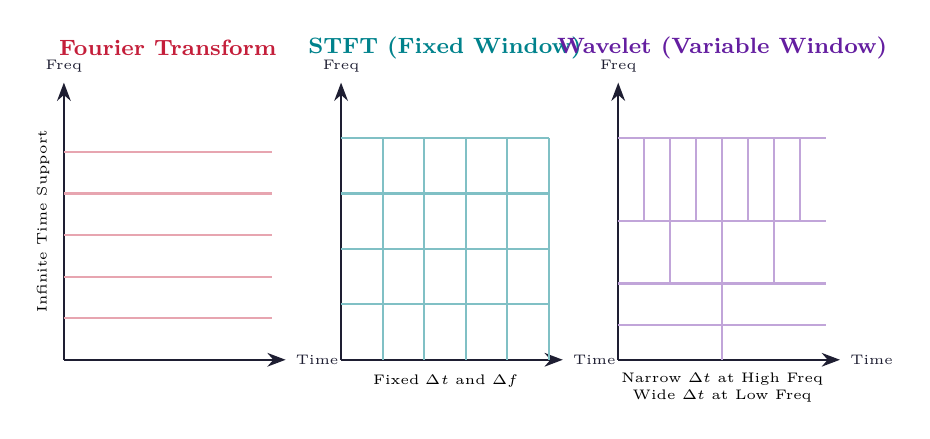
\begin{tikzpicture}[scale=0.88]
  % Fourier Transform Grid
  \node[font=\footnotesize\bfseries, color=myred] at (1.5,4.5) {Fourier Transform};
  \draw[arrow] (0,0) -- (3.2,0) node[right, font=\tiny] {Time};
  \draw[arrow] (0,0) -- (0,4) node[above, font=\tiny] {Freq};
  \foreach \x in {0.6, 1.2, 1.8, 2.4, 3.0} {
    \draw[line, color=myred!40] (0,\x) -- (3.0,\x);
  }
  \node[font=\tiny, rotate=90] at (-0.3, 2) {Infinite Time Support};

  % STFT Grid
  \node[font=\footnotesize\bfseries, color=myteal] at (5.5,4.5) {STFT (Fixed Window)};
  \draw[arrow] (4.0,0) -- (7.2,0) node[right, font=\tiny] {Time};
  \draw[arrow] (4.0,0) -- (4.0,4) node[above, font=\tiny] {Freq};
  \foreach \x in {0.8, 1.6, 2.4, 3.2} {
    \draw[line, color=myteal!50] (4.0,\x) -- (7.0,\x);
  }
  \foreach \y in {4.6, 5.2, 5.8, 6.4, 7.0} {
    \draw[line, color=myteal!50] (\y, 0) -- (\y, 3.2);
  }
  \node[font=\tiny] at (5.5, -0.3) {Fixed $\Delta t$ and $\Delta f$};

  % Wavelet Grid
  \node[font=\footnotesize\bfseries, color=mypurple] at (9.5,4.5) {Wavelet (Variable Window)};
  \draw[arrow] (8.0,0) -- (11.2,0) node[right, font=\tiny] {Time};
  \draw[arrow] (8.0,0) -- (8.0,4) node[above, font=\tiny] {Freq};
  
  % Dyadic divisions
  \draw[line, color=mypurple!40] (8.0, 0.5) -- (11.0, 0.5);
  \draw[line, color=mypurple!40] (8.0, 1.1) -- (11.0, 1.1);
  \draw[line, color=mypurple!40] (8.0, 2.0) -- (11.0, 2.0);
  \draw[line, color=mypurple!40] (8.0, 3.2) -- (11.0, 3.2);
  
  % Vertical lines
  \draw[line, color=mypurple!40] (9.5, 0) -- (9.5, 3.2);
  \draw[line, color=mypurple!40] (8.75, 1.1) -- (8.75, 3.2);
  \draw[line, color=mypurple!40] (10.25, 1.1) -- (10.25, 3.2);
  \draw[line, color=mypurple!40] (8.375, 2.0) -- (8.375, 3.2);
  \draw[line, color=mypurple!40] (9.125, 2.0) -- (9.125, 3.2);
  \draw[line, color=mypurple!40] (9.875, 2.0) -- (9.875, 3.2);
  \draw[line, color=mypurple!40] (10.625, 2.0) -- (10.625, 3.2);
  
  \node[font=\tiny, align=center] at (9.5, -0.4) {Narrow $\Delta t$ at High Freq\\Wide $\Delta t$ at Low Freq};
\end{tikzpicture}
\end{tcolorbox}

% ===============================================================================
\section{Classification of Continuous and Discrete Wavelet Transforms}
% ===============================================================================

Wavelet transforms are classified based on how the scaling parameter $a$ and translation parameter $b$ are sampled:

\begin{enumerate}[leftmargin=*, itemsep=4pt]
  \item \textbf{Continuous Wavelet Transform (CWT):} The parameters $a$ and $b$ vary continuously over $\mathbb{R} \setminus \{0\}$ and $\mathbb{R}$ respectively. This maps a 1D time-domain signal to a 2D time-scale plane, generating a highly redundant representation. It is ideal for signal analysis, singularity detection, and scientific research.
  \item \textbf{Discrete Wavelet Transform (DWT):} The parameters $a$ and $b$ are sampled discretely. Typically, a \textbf{dyadic grid} is used:
        $$a = 2^j, \quad b = k 2^j, \quad j, k \in \mathbb{Z}$$
        This eliminates representation redundancy, allowing for an orthogonal basis decomposition. It is highly efficient for data compression (e.g. JPEG 2000), denoising, and digital hardware implementation.
\end{enumerate}

\par\noindent
{\renewcommand{\arraystretch}{1.4}%
\begin{tabularx}{\linewidth}{|B{3.5cm}|Y|Y|}
\hline
\textbf{Feature} & \textbf{Continuous Wavelet (CWT)} & \textbf{Discrete Wavelet (DWT)} \\
\hline
\textbf{Scaling ($a$) \& Shift ($b$)} & Continuously variable ($a,b \in \mathbb{R}$). & Discretely sampled ($a=2^j, b=k2^j$). \\
\hline
\textbf{Redundancy} & High (infinite overlapping coefficients). & None (orthogonal / non-redundant). \\
\hline
\textbf{Reconstruction} & Uses stable double integral. & Uses digital filter banks (perfect reconstruction). \\
\hline
\textbf{Best Use Case} & Singularity parsing, physics, and analysis. & Signal compression, denoising, and coding. \\
\hline
\end{tabularx}}

% ===============================================================================
\section{Developments in Wavelet Theory Applications}
% ===============================================================================

Since its formalization, wavelet theory has seen rapid developments and applications across various engineering and scientific fields:
\begin{itemize}[leftmargin=*, itemsep=4pt]
  \item \textbf{Seismic Signal Processing:} Jean Morlet's initial development for processing geophysics reflection waves to localize underground oil deposits.
  \item \textbf{Data \& Image Compression:} Standardized in JPEG 2000 (DWT) and FBI fingerprint databases, allowing high-quality storage with minimal memory.
  \item \textbf{Biomedical Engineering:} Analyzing ECG (electrocardiogram) and EEG (electroencephalogram) signals for transient spike detection (such as epilepsy seizures) and denoising.
  \item \textbf{Communication Systems:} Subcarrier modulation schemes like Discrete Wavelet Multi-Tone (DWMT) to suppress inter-carrier interference in multicarrier systems.
\end{itemize}

\newpage
% ===============================================================================
\begin{center}
  {\large\bfseries\color{myred} Quick Revision --- Module 1}\\[3pt]
  {\small\color{mydark} Introduction to Wavelet Theory $|$ PE-EC703C}
\end{center}
\noindent{\color{myred}\rule{\linewidth}{1.2pt}}
\vspace{4pt}
% ===============================================================================

\begin{tcolorbox}[formulabox, title={\textbf{Key Time-Frequency Equations}}]
\renewcommand{\arraystretch}{1.35}
\begin{tabularx}{\linewidth}{B{5.0cm} X}
Fourier Transform & $X(f) = \int_{-\infty}^{\infty} x(t) e^{-j 2\pi f t} dt$ \\[4pt]
Short-Time FT (STFT) & $STFT_x(\tau, f) = \int_{-\infty}^{\infty} x(t) w^*(t - \tau) e^{-j 2\pi f t} dt$ \\[4pt]
Heisenberg Uncertainty & $\Delta t \cdot \Delta f \ge \frac{1}{4\pi} \quad$ (Limits simultaneous time-frequency resolution)
\end{tabularx}
\tcbset{after={\color{black}}}
\end{tcolorbox}

\begin{tcolorbox}[defbox, title={\textbf{One-Line Definitions}}]
\begin{itemize}[leftmargin=*, itemsep=3.5pt]
  \item \textbf{Wavelet:} A localized, oscillatory wave-like function of finite duration with a zero mean value.
  \item \textbf{Fourier Transform:} Spectral mapping with infinite time support, providing no temporal location details.
  \item \textbf{STFT:} Time-frequency mapping that uses a fixed window width, imposing rigid time-frequency resolutions.
  \item \textbf{Multi-resolution Approach:} Analysis method that analyzes signals with narrow windows at high frequencies and wide windows at low frequencies.
  \item \textbf{CWT:} Wavelet transform where parameters vary continuously, providing a redundant, high-resolution representation.
  \item \textbf{DWT:} Wavelet transform where parameters are sampled on a discrete grid, providing an orthogonal representation.
\end{itemize}
\end{tcolorbox}

\begin{tcolorbox}[exambox, title={\textbf{Frequently Asked / Viva Questions}}]
\begin{enumerate}[topsep=0pt, label=\textbf{Q\arabic*.}, itemsep=5pt]
  \item \Q{Why can the Fourier Transform not analyze non-stationary signals?}
        The Fourier Transform integrates over all time ($-\infty$ to $\infty$), meaning it assumes the signal's spectral components do not change over time. It has no time localization, so it cannot identify *when* a transient event or change in frequency occurs.

  \item \Q{How does the Short-Time Fourier Transform (STFT) attempt to fix the limitations of the Fourier Transform?}
        The STFT divides the signal into short segments by multiplying it with a sliding window function. The Fourier Transform is then computed for each segment, providing a time-frequency spectrogram.

  \item \Q{What is the drawback of the STFT?}
        The STFT uses a fixed window size for all frequencies. Due to Heisenberg's Uncertainty Principle ($\Delta t \cdot \Delta f \ge 1/4\pi$), a narrow window gives good time resolution but poor frequency resolution, while a wide window does the opposite.

  \item \Q{How do Wavelets resolve the resolution trade-off of the STFT?}
        Wavelets use variable-width windows: narrow windows (small scales) at high frequencies for capturing rapid transitions, and wide windows (large scales) at low frequencies for capturing steady long-term behaviors.

  \item \Q{What is the main difference between CWT and DWT in terms of redundancy and representation?}
        CWT translates and scales the mother wavelet continuously, leading to high redundancy and overlapping information, making it best for signal analysis. DWT samples parameters on a discrete dyadic grid, yielding a non-redundant orthogonal representation that is highly efficient for data compression.
\end{enumerate}
\end{tcolorbox}

\begin{tcolorbox}[tikzbox, title={\textbf{Time-Frequency Analysis Features}}]
\par\noindent
{\renewcommand{\arraystretch}{1.4}%
\begin{tabularx}{\linewidth}{|B{3.2cm}|Y|Y|Y|}
\hline
\textbf{Feature} & \textbf{Fourier Transform (FT)} & \textbf{Short-Time FT (STFT)} & \textbf{Wavelet Transform} \\
\hline
\textbf{Time Resolution} & None (integrates over all time). & Fixed (determined by window width). & Variable (excellent at high frequencies). \\
\hline
\textbf{Freq Resolution} & Perfect (at all frequencies). & Fixed (determined by window width). & Variable (excellent at low frequencies). \\
\hline
\textbf{Window Shape} & Infinite ($e^{-j 2\pi f t}$). & Fixed envelope ($w(t)$). & Scaled mother wavelet ($\psi(t/a)$). \\
\hline
\textbf{Best Use Case} & Stationary signals. & Quasi-stationary signals. & Non-stationary/transient signals. \\
\hline
\end{tabularx}}
\end{tcolorbox}


% -- Module 2 -----------------------------------------------------------------
\modulestart{2}{Continuous Time Wavelets \& Definition of CWT}

\section{Continuous Time Wavelets \& Definition of CWT}
% ===============================================================================

The Continuous Wavelet Transform (CWT) maps a 1D time-domain signal into a 2D time-scale plane, allowing localized spectral analysis.

\begin{tcolorbox}[defbox, title={\textbf{Definition of CWT}}]
The \textbf{Continuous Wavelet Transform (CWT)} of a continuous-time signal $x(t) \in L^2(\mathbb{R})$ is the correlation of the signal with a scaled and translated version of a mother wavelet function $\psi(t)$:
$$CWT_x(a, b) = \frac{1}{\sqrt{|a|}} \int_{-\infty}^{\infty} x(t) \psi^*\left(\frac{t-b}{a}\right) dt$$
where:
\begin{itemize}[leftmargin=*, itemsep=2.5pt, topsep=3pt]
  \item $a \in \mathbb{R} \setminus \{0\}$ is the \textbf{scale parameter} (controls compression/dilation).
  \item $b \in \mathbb{R}$ is the \textbf{translation parameter} (controls shift along the time axis).
  \item $\psi(t)$ is the \textbf{mother wavelet}, and $\psi^*(t)$ denotes its complex conjugate.
  \item $\frac{1}{\sqrt{|a|}}$ is the normalization factor ensuring energy is invariant across scales.
\end{itemize}
\end{tcolorbox}

% ===============================================================================
\section{Scaling and Translation Parameters}
% ===============================================================================

\begin{itemize}[leftmargin=*, itemsep=4pt]
  \item \textbf{Scaling ($a$):} Scaling either dilates (stretches) or compresses the mother wavelet:
  \begin{itemize}[leftmargin=*, itemsep=2pt, topsep=2pt]
    \item \textbf{Large scale ($|a| > 1$):} Wavelet is dilated, representing a low-frequency, long-duration window (captures coarse features).
    \item \textbf{Small scale ($|a| < 1$):} Wavelet is compressed, representing a high-frequency, short-duration window (captures fine details and transients).
  \end{itemize}
  \item \textbf{Translation ($b$):} Moves the wavelet along the time axis. It indicates the time center of the window.
\end{itemize}

% ===============================================================================
\section{Constant Q-Factor Filtering Interpretation \& Time-Frequency Resolution}
% ===============================================================================

The ratio of the center frequency $f_c$ of a filter to its bandwidth $\Delta f$ is defined as the \textbf{Quality Factor (Q-factor)}:
$$Q = \frac{f_c}{\Delta f}$$
In CWT, compressing the wavelet in time by $a$ stretches its Fourier spectrum by $1/a$. Thus, center frequency and bandwidth scale proportionally:
$$f_c(a) = \frac{f_c(1)}{a}, \quad \Delta f(a) = \frac{\Delta f(1)}{a} \implies Q = \frac{f_c(a)}{\Delta f(a)} = \text{Constant}$$
Hence, the CWT behaves as a \textbf{constant-Q bandpass filter bank}.

\begin{tcolorbox}[tikzbox, title={Wavelet Dilation and Compression}]
\centering
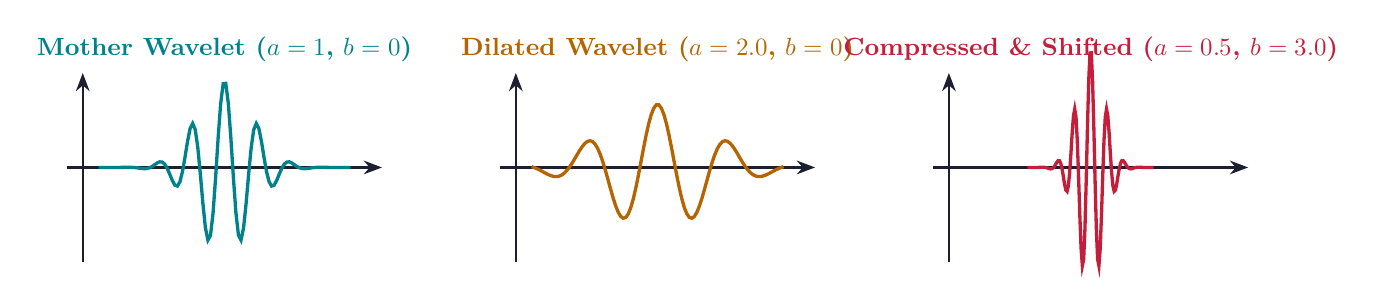
\begin{tikzpicture}
  % Mother Wavelet
  \draw[arrow] (0,-1) -- (4,-1);
  \draw[arrow] (0.2,-2.2) -- (0.2,0.2);
  \draw[line, color=myteal, line width=1.2pt, domain=0.4:3.6, samples=100] 
    plot (\x, {-1 + 1.1*exp(-(\x-2)^2/0.25)*cos(deg(15*(\x-2)))});
  \node[font=\small\bfseries, color=myteal] at (2,0.5) {Mother Wavelet ($a=1$, $b=0$)};

  % Dilated (Large Scale)
  \draw[arrow] (5.5,-1) -- (9.5,-1);
  \draw[arrow] (5.7,-2.2) -- (5.7,0.2);
  \draw[line, color=myamber, line width=1.2pt, domain=5.9:9.1, samples=100] 
    plot (\x, {-1 + 0.8*exp(-(\x-7.5)^2/0.9)*cos(deg(7*(\x-7.5)))});
  \node[font=\small\bfseries, color=myamber] at (7.5,0.5) {Dilated Wavelet ($a=2.0$, $b=0$)};

  % Compressed and Translated
  \draw[arrow] (11,-1) -- (15,-1);
  \draw[arrow] (11.2,-2.2) -- (11.2,0.2);
  \draw[line, color=myred, line width=1.2pt, domain=12.2:13.8, samples=100] 
    plot (\x, {-1 + 1.5*exp(-(\x-13)^2/0.06)*cos(deg(30*(\x-13)))});
  \node[font=\small\bfseries, color=myred] at (13,0.5) {Compressed \& Shifted ($a=0.5$, $b=3.0$)};
\end{tikzpicture}
\end{tcolorbox}

% ===============================================================================
\section{Mathematical Properties of CWT}
% ===============================================================================

\subsection{CWT as a Linear Operator}
The CWT is a \textbf{linear operator}. If $x(t) = c_1 x_1(t) + c_2 x_2(t)$, then:
$$CWT_x(a, b) = c_1 CWT_{x_1}(a, b) + c_2 CWT_{x_2}(a, b)$$

\subsection{Admissibility Condition}
For a function $\psi(t)$ to be a valid mother wavelet, it must satisfy the \textbf{admissibility condition}:
$$C_{\psi} = \int_{-\infty}^{\infty} \frac{|\Psi(f)|^2}{|f|} df < \infty$$
where $\Psi(f)$ is the Fourier transform of $\psi(t)$.
\begin{itemize}[leftmargin=*, itemsep=3pt]
  \item \textbf{Consequence:} For the integral to be finite, $\Psi(0) = 0$. This implies:
  $$\int_{-\infty}^{\infty} \psi(t) dt = 0$$
  The average value (or DC component) of a wavelet must be \textbf{zero}. It must oscillate above and below the zero axis.
\end{itemize}

\subsection{Inverse Continuous Wavelet Transform}
If the admissibility condition $C_{\psi} < \infty$ is met, the signal $x(t)$ can be reconstructed from its wavelet coefficients $CWT_x(a, b)$ via the inverse CWT formula:
$$x(t) = \frac{1}{C_{\psi}} \int_{-\infty}^{\infty} \int_{-\infty}^{\infty} CWT_x(a, b) \frac{1}{\sqrt{|a|}} \psi\left(\frac{t-b}{a}\right) \frac{da db}{a^2}$$

\subsection{Energy Conservation (Parseval's Relation)}
The wavelet transform preserves energy. If $x(t) \in L^2(\mathbb{R})$, then:
$$\int_{-\infty}^{\infty} |x(t)|^2 dt = \frac{1}{C_{\psi}} \int_{-\infty}^{\infty} \int_{-\infty}^{\infty} |CWT_x(a, b)|^2 \frac{da db}{a^2}$$

\newpage
% ===============================================================================
\begin{center}
  {\large\bfseries\color{myred} Quick Revision --- Module 2}\\[3pt]
  {\small\color{mydark} Continuous Wavelet Transform (CWT) $|$ PE-EC703C}
\end{center}
\noindent{\color{myred}\rule{\linewidth}{1.2pt}}
\vspace{4pt}
% ===============================================================================

\begin{tcolorbox}[formulabox, title={\textbf{Key Wavelet Equations}}]
\renewcommand{\arraystretch}{1.35}
\begin{tabularx}{\linewidth}{B{5.0cm} X}
Continuous Wavelet Transform & $CWT_x(a, b) = \frac{1}{\sqrt{|a|}} \int_{-\infty}^{\infty} x(t) \psi^*\left(\frac{t-b}{a}\right) dt$ \\[4pt]
Admissibility Condition & $C_{\psi} = \int_{-\infty}^{\infty} \frac{|\Psi(f)|^2}{|f|} df < \infty \quad \implies \int_{-\infty}^{\infty} \psi(t) dt = 0$ \\[4pt]
Inverse Wavelet Transform & $x(t) = \frac{1}{C_{\psi}} \int_{-\infty}^{\infty} \int_{-\infty}^{\infty} CWT_x(a, b) \frac{1}{\sqrt{|a|}} \psi\left(\frac{t-b}{a}\right) \frac{da db}{a^2}$ \\[4pt]
Constant Q-Factor & $Q = \frac{f_c}{\Delta f} = \text{Constant} \quad$ (Proportional frequency/bandwidth scaling)
\end{tabularx}
\tcbset{after={\color{black}}}
\end{tcolorbox}

\begin{tcolorbox}[defbox, title={\textbf{One-Line Definitions}}]
\begin{itemize}[leftmargin=*, itemsep=3.5pt]
  \item \textbf{CWT:} The correlation of a continuous-time signal with a continuously scaled and translated mother wavelet.
  \item \textbf{Scale Parameter ($a$):} Controls the compression (small $a$, high frequency) or dilation (large $a$, low frequency) of a wavelet.
  \item \textbf{Translation Parameter ($b$):} Determines the temporal location of the wavelet window center along the time axis.
  \item \textbf{Constant Q-Factor:} Quality factor $Q = f_c/\Delta f$ remains constant across scales, behaving as a logarithmic bandpass filter bank.
  \item \textbf{Admissibility Condition:} A mathematical constraint requiring a wavelet's DC component to be zero for reconstruction to be possible.
  \item \textbf{Mother Wavelet:} The prototype wavelet function used to generate all shifted and scaled daughter wavelets.
\end{itemize}
\end{tcolorbox}

\begin{tcolorbox}[exambox, title={\textbf{Frequently Asked / Viva Questions}}]
\begin{enumerate}[topsep=0pt, label=\textbf{Q\arabic*.}, itemsep=5pt]
  \item \Q{State the physical meaning of the scale parameter '$a$'.}
        Scale '$a$' is inversely proportional to frequency. A small scale ($a < 1$) compresses the wavelet, corresponding to high-frequency transients. A large scale ($a > 1$) dilates the wavelet, corresponding to slow-varying low-frequency components.

  \item \Q{What is the significance of the admissibility condition?}
        The admissibility condition ensures that the wavelet does not carry a DC component ($\int_{-\infty}^{\infty} \psi(t) dt = 0$). This guarantees that the inverse wavelet transform exists and enables perfect reconstruction of the signal.

  \item \Q{Explain the constant Q-factor filtering property of the CWT.}
        In CWT, as scale $a$ changes, the center frequency and bandwidth of the wavelet filter change proportionally. Since $Q = f_c/\Delta f$, the quality factor remains constant across all scales, behaving as a logarithmic bandpass filter bank.

  \item \Q{What is the difference between Gabor transform and Wavelet transform?}
        The Gabor transform is a special case of STFT using a Gaussian window. It uses a fixed window envelope across all frequencies. The Wavelet transform uses a scaled envelope that compresses at higher frequencies and expands at lower frequencies.
\end{enumerate}
\tcbset{after={\color{black}}}
\end{tcolorbox}


% -- Module 3 -----------------------------------------------------------------
\modulestart{3}{Multi-resolution Analysis (MRA) Framework}

\section{Multi-resolution Analysis (MRA) Framework}
% ===============================================================================

\begin{tcolorbox}[defbox, title={\textbf{Definition of Multi-resolution Analysis}}]
\textbf{Multi-resolution Analysis (MRA)} is a mathematical framework developed by Mallat and Meyer to construct orthonormal wavelet bases. It represents a continuous-time signal $x(t) \in L^2(\mathbb{R})$ as a limit of successive approximations, each representing a different resolution level.
\end{tcolorbox}

\subsection{Nested Vector Subspaces}
The MRA is characterized by a sequence of closed nested linear vector subspaces $\{V_j\}_{j=-\infty}^{\infty}$ of the Hilbert space $L^2(\mathbb{R})$:
$$\dots \subset V_{-2} \subset V_{-1} \subset V_0 \subset V_1 \subset V_2 \subset \dots \subset L^2(\mathbb{R})$$
where:
\begin{itemize}[leftmargin=*, itemsep=3.5pt]
  \item Each subspace $V_j$ corresponds to a specific \textbf{resolution level} (with larger indices $j$ representing finer details/sampling rates).
  \item Any signal in $V_j$ is also contained in the next finer subspace $V_{j+1}$.
\end{itemize}

\subsection{The Five Core MRA Axioms}
A family of subspaces $\{V_j\}_{j\in\mathbb{Z}}$ constitutes an MRA of $L^2(\mathbb{R})$ if the following mathematical axioms are satisfied:
\begin{enumerate}[leftmargin=*, itemsep=4pt]
  \item \textbf{Containment (Monotonicity):} $V_j \subset V_{j+1}$ for all $j \in \mathbb{Z}$.
  \item \textbf{Completeness (Separation):} The intersection of all subspaces contains only the zero function:
$$\bigcap_{j=-\infty}^{\infty} V_j = \{0\}$$
  \item \textbf{Density:} The union of all subspaces is dense in $L^2(\mathbb{R})$ (any signal can be approximated to arbitrary precision):
$$\overline{\bigcup_{j=-\infty}^{\infty} V_j} = L^2(\mathbb{R})$$
  \item \textbf{Scaling Similarity (Scale Invariance):} Scaling a function in time by a factor of 2 shifts it to the adjacent subspace:
$$f(t) \in V_j \iff f(2t) \in V_{j+1}$$
  \item \textbf{Translation Invariance (Shift Invariance):} Shifting a function in $V_0$ by an integer step remains in $V_0$:
$$f(t) \in V_0 \iff f(t-k) \in V_0 \quad \text{for all } k \in \mathbb{Z}$$
\end{enumerate}

\newpage
\begin{tcolorbox}[tikzbox, title={Nested Vector Subspaces Hierarchy}]
\centering
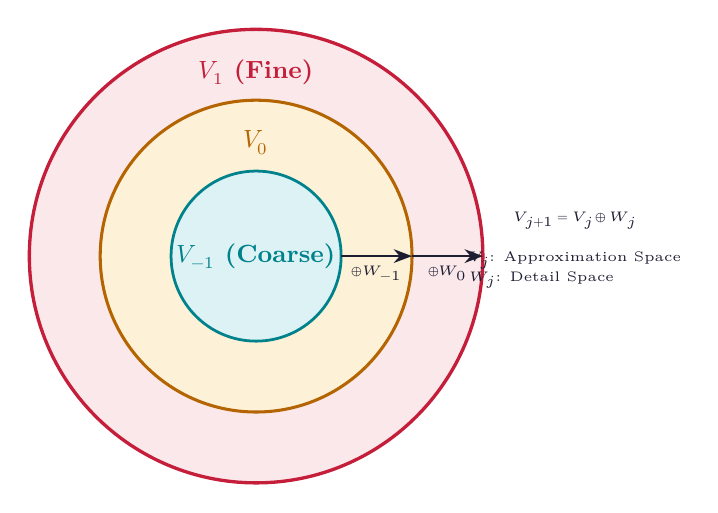
\begin{tikzpicture}[scale=0.9]
  % Nested circles
  \draw[draw=myred, fill=hdrred, line width=1.2pt] (0,0) circle (3.2);
  \draw[draw=myamber, fill=hdramber, line width=1.1pt] (0,0) circle (2.2);
  \draw[draw=myteal, fill=hdrteal, line width=1.0pt] (0,0) circle (1.2);
  
  % Labels
  \node[color=myteal, font=\small\bfseries] at (0, 0) {$V_{-1}$ (Coarse)};
  \node[color=myamber, font=\small\bfseries] at (0, 1.6) {$V_0$};
  \node[color=myred, font=\small\bfseries] at (0, 2.6) {$V_1$ (Fine)};
  
  % Detail space mapping
  \draw[arrow, color=mydark] (1.2, 0) -- (2.2, 0) node[midway, below, font=\tiny] {$\oplus W_{-1}$};
  \draw[arrow, color=mydark] (2.2, 0) -- (3.2, 0) node[midway, below, font=\tiny] {$\oplus W_0$};
  
  \node[font=\tiny\bfseries, color=mydark] at (4.5, 0.5) {$V_{j+1} = V_j \oplus W_j$};
  \node[font=\tiny, color=mydark, align=left] at (4.5, -0.2) {$V_j$: Approximation Space\\$W_j$: Detail Space};
\end{tikzpicture}
\end{tcolorbox}

% ===============================================================================
\section{Scaling Function and Wavelet Function}
% ===============================================================================

An MRA is completely defined by its \textbf{scaling function $\phi(t)$} (also known as the \textbf{Father Wavelet}).

\subsection{The Dilation (Refinement) Equation}
Because $\phi(t) \in V_0 \subset V_1$, and the set $\{\sqrt{2}\phi(2t-k)\}_{k\in\mathbb{Z}}$ forms an orthonormal basis for $V_1$, the scaling function can be expanded as a linear combination of scaled and shifted copies of itself. This is the \textbf{refinement equation} (or \textbf{dilation equation}):
$$\phi(t) = \sqrt{2} \sum_{k=-\infty}^{\infty} h_0[k] \phi(2t - k)$$
where $h_0[k]$ are the \textbf{scaling filter coefficients} (low-pass filter).

\subsection{Detail Spaces ($W_j$) and the Wavelet Function}
The approximation space $V_{j+1}$ has finer resolution than $V_j$. The missing information between them is represented by the \textbf{detail space $W_j$}, defined as the orthogonal complement of $V_j$ in $V_{j+1}$:
$$V_{j+1} = V_j \oplus W_j \quad \text{where } V_j \perp W_j$$
By repeating this decomposition:
$$V_{j+1} = V_{j-1} \oplus W_{j-1} \oplus W_j = V_0 \oplus \bigoplus_{i=0}^{j} W_i$$
To span the detail spaces, we define the \textbf{wavelet function $\psi(t)$} (the \textbf{Mother Wavelet}), which can also be written in terms of the scaling function at the next scale:
$$\psi(t) = \sqrt{2} \sum_{k=-\infty}^{\infty} h_1[k] \phi(2t - k)$$
where $h_1[k]$ are the \textbf{wavelet filter coefficients} (high-pass filter).

% ===============================================================================
\section{The Haar Wavelet System}
% ===============================================================================

The \textbf{Haar system} is the oldest and simplest example of an MRA.

\subsection{Haar Scaling Function (Father Wavelet)}
The Haar scaling function $\phi(t)$ is a simple unit step box function:
$$\phi(t) = \begin{cases} 1 & 0 \le t < 1 \\ 0 & \text{otherwise} \end{cases}$$
Its refinement equation is:
$$\phi(t) = \phi(2t) + \phi(2t-1)$$
Comparing with the general dilation equation $\phi(t) = \sqrt{2}[h_0[0]\phi(2t) + h_0[1]\phi(2t-1)]$, the Haar scaling filter coefficients are:
$$h_0[0] = \frac{1}{\sqrt{2}}, \quad h_0[1] = \frac{1}{\sqrt{2}} \quad (\text{all other } h_0[k] = 0)$$

\subsection{Haar Wavelet Function (Mother Wavelet)}
The Haar wavelet $\psi(t)$ is defined as:
$$\psi(t) = \begin{cases} 1 & 0 \le t < 0.5 \\ -1 & 0.5 \le t < 1 \\ 0 & \text{otherwise} \end{cases}$$
Its refinement equation is:
$$\psi(t) = \phi(2t) - \phi(2t-1)$$
Thus, the Haar wavelet filter coefficients are:
$$h_1[0] = \frac{1}{\sqrt{2}}, \quad h_1[1] = -\frac{1}{\sqrt{2}} \quad (\text{all other } h_1[k] = 0)$$

\begin{tcolorbox}[tikzbox, title={Haar Scaling Function and Wavelet Plots}]
\centering
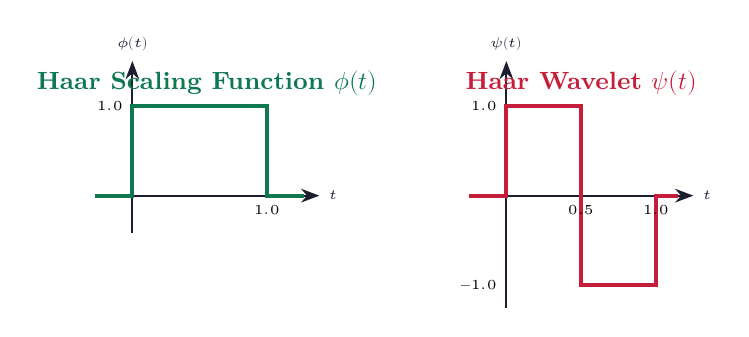
\begin{tikzpicture}[scale=0.95]
  % Scaling Function Plot
  \draw[arrow] (-0.5,0) -- (2.5,0) node[right, font=\tiny] {$t$};
  \draw[arrow] (0,-0.5) -- (0,1.8) node[above, font=\tiny] {$\phi(t)$};
  \draw[line, color=mygreen, line width=1.5pt] (-0.5,0) -- (0,0) -- (0,1.2) -- (1.8,1.2) -- (1.8,0) -- (2.3,0);
  \node[left, font=\tiny] at (0,1.2) {$1.0$};
  \node[below, font=\tiny] at (1.8,0) {$1.0$};
  \node[font=\small\bfseries, color=mygreen] at (1,1.5) {Haar Scaling Function $\phi(t)$};

  % Wavelet Function Plot
  \draw[arrow] (4.5,0) -- (7.5,0) node[right, font=\tiny] {$t$};
  \draw[arrow] (5.0,-1.5) -- (5.0,1.8) node[above, font=\tiny] {$\psi(t)$};
  \draw[line, color=myred, line width=1.5pt] 
    (4.5,0) -- (5.0,0) -- (5.0,1.2) -- (6.0,1.2) -- (6.0,-1.2) -- (7.0,-1.2) -- (7.0,0) -- (7.3,0);
  \node[left, font=\tiny] at (5.0,1.2) {$1.0$};
  \node[left, font=\tiny] at (5.0,-1.2) {$-1.0$};
  \node[below, font=\tiny] at (6.0,0) {$0.5$};
  \node[below, font=\tiny] at (7.0,0) {$1.0$};
  \node[font=\small\bfseries, color=myred] at (6,1.5) {Haar Wavelet $\psi(t)$};
\end{tikzpicture}
\end{tcolorbox}

\subsection{Haar Wavelet Decomposition Example}
Consider a discrete-time signal $x = [c_1, c_2]$ representing values in space $V_1$.
\begin{enumerate}[leftmargin=*, itemsep=4.5pt]
  \item \textbf{Approximation coefficient} (Low-pass projection in $V_0$):
        $$a_1 = \frac{c_1 + c_2}{\sqrt{2}}$$
  \item \textbf{Detail coefficient} (High-pass projection in $W_0$):
        $$d_1 = \frac{c_1 - c_2}{\sqrt{2}}$$
\end{enumerate}
The Haar transform maps $[c_1, c_2] \to [a_1, d_1]$. It decomposes the signal into its local mean (coarse trend) and local difference (detail fluctuation).

\subsection{Haar Wavelet Packets and Applications}
A standard Haar DWT only decomposes the low-pass approximation coefficients ($a_j$) recursively. A \textbf{Haar Wavelet Packet} decomposition recursively filters both the approximation ($a_j$) and the detail ($d_j$) coefficients at each level, yielding a full balanced binary tree.

\subsubsection{Recursive Generation of Haar Wavelet Packets}
Let $W_0(t) = \phi(t)$ be the Haar scaling function and $W_1(t) = \psi(t)$ be the Haar wavelet function. The higher-order wavelet packet functions $W_n(t)$ for $n \ge 0$ are recursively defined by:
$$W_{2n}(t) = \sum_{k=0}^{1} h_0[k] W_n(2t - k) = \frac{1}{\sqrt{2}} \left[ W_n(2t) + W_n(2t-1) \right]$$
$$W_{2n+1}(t) = \sum_{k=0}^{1} h_1[k] W_n(2t - k) = \frac{1}{\sqrt{2}} \left[ W_n(2t) - W_n(2t-1) \right]$$
For example, starting from the first level:
\begin{itemize}[leftmargin=*, itemsep=2pt]
  \item $W_2(t)$ is generated from the low-pass projection of $W_1(t)$, representing a high-frequency approximation packet.
  \item $W_3(t)$ is generated from the high-pass projection of $W_1(t)$, representing a high-frequency detail packet.
\end{itemize}

\subsubsection{Applications of Haar Wavelet Packets}
Due to their simple step-like structure and ease of computational implementation, Haar wavelet packets are widely used in:
\begin{itemize}[leftmargin=*, itemsep=3.5pt]
  \item \textbf{Transient Signal Detection:} The localized rectangular support of Haar packets makes them highly sensitive to sudden spikes, edges, and discontinuities in signals.
  \item \textbf{High-Frequency Feature Extraction:} By decomposing the high-frequency bands recursively, Haar packets capture structural texture details in images that standard DWT skips.
  \item \textbf{Real-Time Low-Power Hardware Implementations:} Since the Haar filter coefficients ($1/\sqrt{2}$) involve simple additions and subtractions, Haar packet transforms are ideal for low-cost hardware implementation on microcontrollers and FPGAs.
\end{itemize}

\newpage
% ===============================================================================
\begin{center}
  {\large\bfseries\color{myred} Quick Revision --- Module 3}\\[3pt]
  {\small\color{mydark} Discrete Wavelet Transform \& MRA $|$ PE-EC703C}
\end{center}
\noindent{\color{myred}\rule{\linewidth}{1.2pt}}
\vspace{4pt}
% ===============================================================================

\begin{tcolorbox}[formulabox, title={\textbf{Key DWT \& MRA Equations}}]
\renewcommand{\arraystretch}{1.35}
\begin{tabularx}{\linewidth}{B{5.0cm} X}
MRA Nested Spaces & $\dots \subset V_{-1} \subset V_0 \subset V_1 \subset V_2 \dots \subset L^2(\mathbb{R})$ \\[4pt]
Scaling Refinement Eq. & $\phi(t) = \sqrt{2} \sum_{k} h_0[k] \phi(2t - k) \quad$ (Father Wavelet) \\[4pt]
Wavelet Refinement Eq. & $\psi(t) = \sqrt{2} \sum_{k} h_1[k] \phi(2t - k) \quad$ (Mother Wavelet) \\[4pt]
Orthogonal Complement & $V_{j+1} = V_j \oplus W_j \quad$ where $V_j \perp W_j$ \\[4pt]
Haar scaling coefficients & $h_0[0] = 1/\sqrt{2}, \quad h_0[1] = 1/\sqrt{2}$ \\[4pt]
Haar wavelet coefficients & $h_1[0] = 1/\sqrt{2}, \quad h_1[1] = -1/\sqrt{2}$
\end{tabularx}
\tcbset{after={\color{black}}}
\end{tcolorbox}

\begin{tcolorbox}[defbox, title={\textbf{One-Line Definitions}}]
\begin{itemize}[leftmargin=*, itemsep=3.5pt]
  \item \textbf{MRA:} A mathematical framework decomposing a signal into nested resolution spaces.
  \item \textbf{Approximation Space ($V_j$):} Subspace containing low-resolution signal trends up to scale $j$.
  \item \textbf{Detail Space ($W_j$):} Subspace containing the localized high-resolution differences between $V_j$ and $V_{j+1}$.
  \item \textbf{Father Wavelet ($\phi(t)$):} The scaling function that spans the approximation spaces.
  \item \textbf{Mother Wavelet ($\psi(t)$):} The wavelet function that spans the detail spaces.
  \item \textbf{Dilation Equation:} A recursive relation defining the scaling function using scaled/shifted copies of itself.
  \item \textbf{Haar Wavelet:} The simplest orthonormal wavelet, represented by an asymmetric step function.
\end{itemize}
\end{tcolorbox}

\begin{tcolorbox}[exambox, title={\textbf{Frequently Asked / Viva Questions}}]
\begin{enumerate}[topsep=0pt, label=\textbf{Q\arabic*.}, itemsep=5pt]
  \item \Q{State the five basic axioms of Multi-resolution Analysis (MRA).}
        The five axioms are: (1) Containment: $V_j \subset V_{j+1}$; (2) Completeness: $\bigcap V_j = \{0\}$; (3) Density: $\overline{\bigcup V_j} = L^2(\mathbb{R})$; (4) Scaling Similarity: $f(t) \in V_j \iff f(2t) \in V_{j+1}$; and (5) Translation Invariance: $f(t) \in V_0 \iff f(t-k) \in V_0$.

  \item \Q{What is the difference between approximation space and detail space?}
        The approximation space ($V_j$) represents the low-frequency, smoothed version of a signal at resolution scale $j$. The detail space ($W_j$) represents the high-frequency difference or fluctuation needed to transition from a coarse scale $V_j$ to a finer scale $V_{j+1}$.

  \item \Q{Write down the refinement/dilation equation for the scaling function.}
        The refinement equation is: $\phi(t) = \sqrt{2} \sum_{k=-\infty}^{\infty} h_0[k] \phi(2t-k)$, where $h_0[k]$ are the scaling filter coefficients. This equation shows that the scaling function is self-similar across scales.

  \item \Q{What are the coefficients of the Haar scaling and wavelet filters?}
        For the Haar scaling filter: $h_0[0] = 1/\sqrt{2}$, $h_0[1] = 1/\sqrt{2}$. For the Haar wavelet filter: $h_1[0] = 1/\sqrt{2}$, $h_1[1] = -1/\sqrt{2}$. All other coefficients are zero.

  \item \Q{Why does the DWT avoid the redundancy of the CWT?}
        The CWT varies the scale $a$ and shift $b$ continuously, creating infinite overlap and redundant representation. The DWT samples the time-scale grid discretely (usually on a dyadic grid: $a = 2^j, b = k \cdot 2^j$), creating an orthogonal, non-redundant representation.

  \item \Q{What is the relation between the scaling function $\phi(t)$ and the wavelet function $\psi(t)$?}
        The scaling function $\phi(t)$ generates the approximation spaces ($V_j$). The wavelet function $\psi(t)$ is orthogonal to $\phi(t)$ and generates the detail spaces ($W_j$). Mathematically, $\psi(t)$ is derived from the scaling function via: $\psi(t) = \sqrt{2} \sum_{k} h_1[k] \phi(2t-k)$.

  \item \Q{What are the drawbacks of the Haar wavelet system?}
        The Haar wavelet is discontinuous in the time domain, which causes poor frequency resolution and spectral leakage. Additionally, it has only one vanishing moment, making it inefficient for compressing smooth signals.
\end{enumerate}
\end{tcolorbox}

\begin{tcolorbox}[tikzbox, title={\textbf{Comparison Table: Approximation vs. Detail Spaces}}]
\par\noindent
{\renewcommand{\arraystretch}{1.4}%
\begin{tabularx}{\linewidth}{|B{3.2cm}|Y|Y|}
\hline
\textbf{Feature} & \textbf{Approximation Space ($V_j$)} & \textbf{Detail Space ($W_j$)} \\
\hline
\textbf{Spanning Basis} & Shifted Scaling Functions: $\{\phi_{j,k}(t)\}$. & Shifted Wavelet Functions: $\{\psi_{j,k}(t)\}$. \\
\hline
\textbf{Spectral Content} & Low-frequency components (trends). & High-frequency components (details/edges). \\
\hline
\textbf{Filtering Operation} & Low-pass filter ($h_0[k]$). & High-pass filter ($h_1[k]$). \\
\hline
\textbf{Relationship} & $V_{j+1} = V_j \oplus W_j$ & $W_j \perp V_j$ and $W_j \perp W_i$ (for $i \neq j$). \\
\hline
\end{tabularx}}
\end{tcolorbox}


% -- Module 4 -----------------------------------------------------------------
\modulestart{4}{2-Channel Filter Banks and Subband Coding}

\section{2-Channel Filter Banks and Subband Coding}
% ===============================================================================

Multi-resolution analysis is implemented in practice using \textbf{digital filter banks}. A \textbf{2-Channel Filter Bank} splits a signal into two subbands (Analysis) and reconstructs it back to a single signal (Synthesis).

\subsection{Analysis and Synthesis Filter Banks}
\begin{enumerate}[leftmargin=*, itemsep=4pt]
  \item \textbf{Analysis Filter Bank (Decomposition):}
        \begin{itemize}[leftmargin=*, itemsep=2.5pt, topsep=2pt]
          \item \textbf{Low-Pass Filter ($H_0(z)$):} Extracts approximation components.
          \item \textbf{High-Pass Filter ($H_1(z)$):} Extracts detail components.
          \item \textbf{Decimation / Downsampling ($\downarrow 2$):} Discards every second sample to maintain the original data rate, yielding subband signals $v_0[n]$ and $v_1[n]$.
        \end{itemize}
  \item \textbf{Synthesis Filter Bank (Reconstruction):}
        \begin{itemize}[leftmargin=*, itemsep=2.5pt, topsep=2pt]
          \item \textbf{Interpolation / Upsampling ($\uparrow 2$):} Inserts a zero between adjacent samples.
          \item \textbf{Low-Pass Filter ($G_0(z)$):} Smooths the upsampled approximation.
          \item \textbf{High-Pass Filter ($G_1(z)$):} Smooths the upsampled detail.
          \item The filtered outputs are summed together to produce the reconstructed signal $\hat{x}[n]$.
        \end{itemize}
\end{enumerate}

\begin{tcolorbox}[tikzbox, title={2-Channel Subband Coder / Filter Bank System}]
\centering
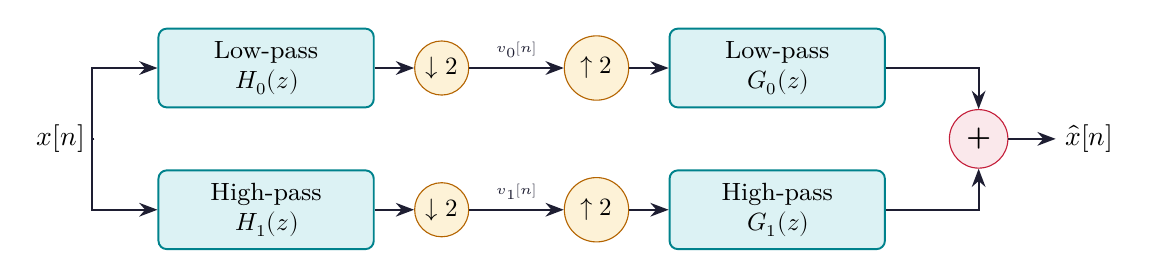
\begin{tikzpicture}[node distance=0.6cm and 0.8cm]
  % Input
  \node (in) {$x[n]$};
  
  % Analysis Filters
  \node[block, right=0.8cm of in, yshift=0.9cm] (h0) {Low-pass\\$H_0(z)$};
  \node[block, right=0.8cm of in, yshift=-0.9cm] (h1) {High-pass\\$H_1(z)$};
  
  % Downsamplers
  \node[circle, draw=myamber, fill=hdramber, right=0.5cm of h0, inner sep=2pt] (d0) {\small $\downarrow 2$};
  \node[circle, draw=myamber, fill=hdramber, right=0.5cm of h1, inner sep=2pt] (d1) {\small $\downarrow 2$};
  
  % Upsamplers
  \node[circle, draw=myamber, fill=hdramber, right=1.2cm of d0] (u0) {\small $\uparrow 2$};
  \node[circle, draw=myamber, fill=hdramber, right=1.2cm of d1] (u1) {\small $\uparrow 2$};
  
  % Synthesis Filters
  \node[block, right=0.5cm of u0] (g0) {Low-pass\\$G_0(z)$};
  \node[block, right=0.5cm of u1] (g1) {High-pass\\$G_1(z)$};
  
  % Summation
  \node[circle, draw=myred, fill=hdrred, right=0.8cm of g0, yshift=-0.9cm] (sum) {\textbf{+}};
  \node[right=0.6cm of sum] (out) {$\hat{x}[n]$};
  
  % Connections
  \draw[arrow] (in) -- ++(0.4,0) |- (h0.west);
  \draw[arrow] (in) -- ++(0.4,0) |- (h1.west);
  \draw[arrow] (h0) -- (d0);
  \draw[arrow] (h1) -- (d1);
  \draw[arrow] (d0) -- (u0) node[midway, above, font=\tiny] {$v_0[n]$};
  \draw[arrow] (d1) -- (u1) node[midway, above, font=\tiny] {$v_1[n]$};
  \draw[arrow] (u0) -- (g0);
  \draw[arrow] (u1) -- (g1);
  \draw[arrow] (g0.east) -| (sum.north);
  \draw[arrow] (g1.east) -| (sum.south);
  \draw[arrow] (sum) -- (out);
\end{tikzpicture}
\end{tcolorbox}

% ===============================================================================
\section{Perfect Reconstruction (PR) Conditions}
% ===============================================================================

Let the $Z$-transform of the reconstructed signal be $\hat{X}(z)$. The input-output relationship of the 2-channel filter bank is:
$$\hat{X}(z) = \frac{1}{2}\left[H_0(z)G_0(z) + H_1(z)G_1(z)\right]X(z) + \frac{1}{2}\left[H_0(-z)G_0(z) + H_1(-z)G_1(z)\right]X(-z)$$
where the term involving $X(-z)$ represents \textbf{aliasing} introduced by downsampling.

\subsection{Aliasing Cancellation Condition}
To completely cancel aliasing, the second term must be zero for all $X(z)$:
$$H_0(-z)G_0(z) + H_1(-z)G_1(z) = 0$$
This is achieved by choosing synthesis filters that mirror the analysis filters:
$$G_0(z) = H_1(-z), \quad G_1(z) = -H_0(-z)$$

\subsection{No Distortion Condition}
After substituting the aliasing cancellation parameters, we require $\hat{x}[n]$ to be a delayed version of the input: $\hat{x}[n] = x[n - d] \implies \hat{X}(z) = z^{-d}X(z)$. This yields the \textbf{no distortion condition}:
$$H_0(z)G_0(z) + H_1(z)G_1(z) = 2z^{-d}$$

\subsection{Orthonormal Quadrature Mirror Filters (QMF)}
In an orthonormal filter bank, the filters must satisfy conjugate symmetry conditions. In the time domain, the relationship is:
$$h_1[k] = (-1)^k h_0[N - 1 - k] \quad (\text{where } N \text{ is the filter length})$$
In the $Z$-domain, this translates to:
$$H_1(z) = z^{-(N-1)}H_0(-z^{-1})$$
This ensures that the filter bank cancels aliasing, has no amplitude distortion, and is orthonormal.

% ===============================================================================
\section{Discrete-Time Multi-resolution Analysis}
% ===============================================================================

To decompose a signal across multiple scales, we cascade the Analysis filter bank in an octave tree structure (the \textbf{Mallat Algorithm}).

\begin{tcolorbox}[tikzbox, title={Wavelet Octave-Band Decomposition Tree (Mallat Algorithm)}]
\centering
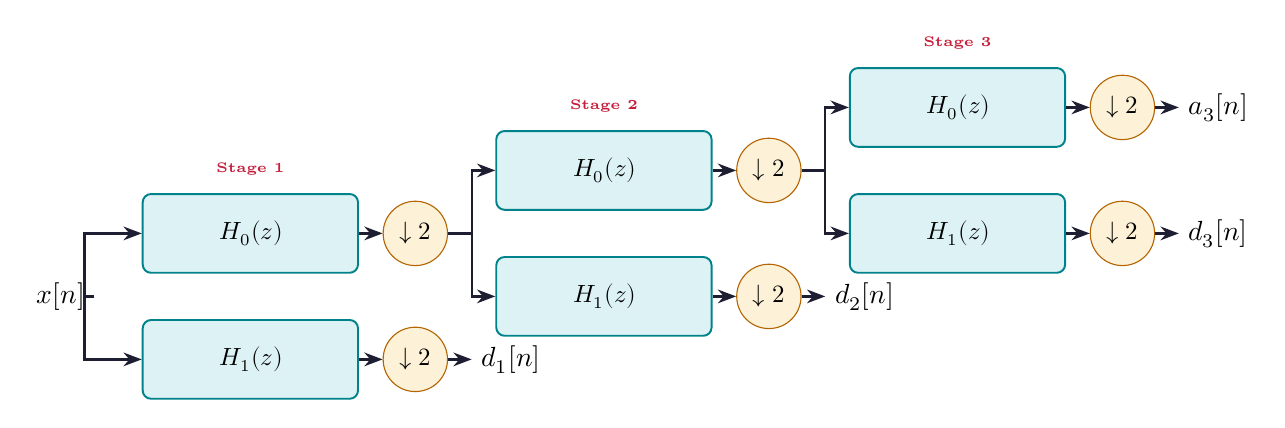
\begin{tikzpicture}[node distance=0.5cm and 0.8cm,
  lbl/.style={font=\tiny\bfseries, color=myred}]
  
  % Level 1
  \node (in) {$x[n]$};
  \node[block, right=0.6cm of in, yshift=0.8cm] (h01) {$H_0(z)$};
  \node[block, right=0.6cm of in, yshift=-0.8cm] (h11) {$H_1(z)$};
  \node[circle, draw=myamber, fill=hdramber, right=0.3cm of h01] (d01) {\small $\downarrow 2$};
  \node[circle, draw=myamber, fill=hdramber, right=0.3cm of h11] (d11) {\small $\downarrow 2$};
  \node[right=0.3cm of d11] (d1) {$d_1[n]$};
  
  % Level 2
  \node[block, right=0.6cm of d01, yshift=0.8cm] (h02) {$H_0(z)$};
  \node[block, right=0.6cm of d01, yshift=-0.8cm] (h12) {$H_1(z)$};
  \node[circle, draw=myamber, fill=hdramber, right=0.3cm of h02] (d02) {\small $\downarrow 2$};
  \node[circle, draw=myamber, fill=hdramber, right=0.3cm of h12] (d12) {\small $\downarrow 2$};
  \node[right=0.3cm of d12] (d2) {$d_2[n]$};
  
  % Level 3
  \node[block, right=0.6cm of d02, yshift=0.8cm] (h03) {$H_0(z)$};
  \node[block, right=0.6cm of d02, yshift=-0.8cm] (h13) {$H_1(z)$};
  \node[circle, draw=myamber, fill=hdramber, right=0.3cm of h03] (d03) {\small $\downarrow 2$};
  \node[circle, draw=myamber, fill=hdramber, right=0.3cm of h13] (d13) {\small $\downarrow 2$};
  \node[right=0.3cm of d03] (a3) {$a_3[n]$};
  \node[right=0.3cm of d13] (d3) {$d_3[n]$};

  % Connections
  \draw[arrow] (in) -- ++(0.3,0) |- (h01.west);
  \draw[arrow] (in) -- ++(0.3,0) |- (h11.west);
  \draw[arrow] (h01) -- (d01);
  \draw[arrow] (h11) -- (d11);
  \draw[arrow] (d11) -- (d1);
  
  \draw[arrow] (d01.east) -- ++(0.3,0) |- (h02.west);
  \draw[arrow] (d01.east) -- ++(0.3,0) |- (h12.west);
  \draw[arrow] (h02) -- (d02);
  \draw[arrow] (h12) -- (d12);
  \draw[arrow] (d12) -- (d2);
  
  \draw[arrow] (d02.east) -- ++(0.3,0) |- (h03.west);
  \draw[arrow] (d02.east) -- ++(0.3,0) |- (h13.west);
  \draw[arrow] (h03) -- (d03);
  \draw[arrow] (h13) -- (d13);
  \draw[arrow] (d03) -- (a3);
  \draw[arrow] (d13) -- (d3);
  
  \node[lbl, above=0.1cm of h01] {Stage 1};
  \node[lbl, above=0.1cm of h02] {Stage 2};
  \node[lbl, above=0.1cm of h03] {Stage 3};
\end{tikzpicture}
\end{tcolorbox}

% ===============================================================================
\section{Orthonormal Wavelet Families}
% ===============================================================================

To compute wavelets from filter coefficients, we use the \textbf{Cascade Algorithm (Refinement)}. By repeatedly upsampling and filtering $h_0[k]$, the scaling function $\phi(t)$ is generated at the limit.

Several standard orthogonal families exist, each offering unique trade-offs:
\begin{enumerate}[leftmargin=*, itemsep=4pt]
  \item \textbf{Daubechies Wavelets (dbN):} Orthonormal, compactly supported wavelets with the maximum number of vanishing moments (equal to $N$, the filter order). This maximizes frequency response sharpness and makes them excellent for compression.
  \item \textbf{Symlets (symN):} Designed by Ingrid Daubechies to be "least asymmetric" versions of the db wavelets, providing near-linear phase characteristics while maintaining orthonormality.
  \item \textbf{Coiflets (coifN):} Scaling functions also have vanishing moments, which improves polynomial approximation accuracy in both scaling and wavelet spaces.
\end{enumerate}

\newpage
% ===============================================================================
\begin{center}
  {\large\bfseries\color{myred} Quick Revision --- Module 4}\\[3pt]
  {\small\color{mydark} MRA Ortho-normal Wavelets \& Filter Banks $|$ PE-EC703C}
\end{center}
\noindent{\color{myred}\rule{\linewidth}{1.2pt}}
\vspace{4pt}
% ===============================================================================

\begin{tcolorbox}[formulabox, title={\textbf{Key Filter Bank Equations}}]
\renewcommand{\arraystretch}{1.35}
\begin{tabularx}{\linewidth}{B{5.0cm} X}
Aliasing Cancellation & $H_0(-z)G_0(z) + H_1(-z)G_1(z) = 0$ \\[4pt]
No Distortion Condition & $H_0(z)G_0(z) + H_1(z)G_1(z) = 2z^{-d}$ \\[4pt]
Synthesis Filters (PR) & $G_0(z) = H_1(-z), \quad G_1(z) = -H_0(-z)$ \\[4pt]
Orthonormal QMF Relation & $h_1[k] = (-1)^k h_0[N - 1 - k] \quad \implies H_1(z) = z^{-(N-1)}H_0(-z^{-1})$ \\[4pt]
Vanishing Moments dbN & $\int_{-\infty}^{\infty} t^p \psi(t) dt = 0 \quad$ for $p = 0, 1, \dots, N-1$
\end{tabularx}
\tcbset{after={\color{black}}}
\end{tcolorbox}

\begin{tcolorbox}[defbox, title={\textbf{One-Line Definitions}}]
\begin{itemize}[leftmargin=*, itemsep=3.5pt]
  \item \textbf{Filter Bank:} A system of parallel digital filters that splits (Analysis) and recombines (Synthesis) a signal.
  \item \textbf{Subband Coding:} Compression technique where a signal is split into frequency bands and coded separately.
  \item \textbf{Decimation ($\downarrow 2$):} Downsampling operation that discards every other sample, compressing the spectrum.
  \item \textbf{Interpolation ($\uparrow 2$):} Upsampling operation that inserts zeros between samples, expanding the spectrum.
  \item \textbf{QMF (Quadrature Mirror Filter):} A filter bank where high-pass and low-pass filters are mirror images across $f_s/4$.
  \item \textbf{Vanishing Moments:} The power to which a wavelet can cancel out polynomial components, aiding signal compression.
  \item \textbf{Cascade Algorithm:} Iterative upsampling/filtering technique used to construct scaling functions from coefficients.
\end{itemize}
\end{tcolorbox}

\begin{tcolorbox}[exambox, title={\textbf{Frequently Asked / Viva Questions}}]
\begin{enumerate}[topsep=0pt, label=\textbf{Q\arabic*.}, itemsep=5pt]
  \item \Q{What are the conditions for Perfect Reconstruction (PR) in a 2-channel filter bank?}
        Perfect reconstruction requires: (1) Aliasing Cancellation: $H_0(-z)G_0(z) + H_1(-z)G_1(z) = 0$, and (2) No Distortion: $H_0(z)G_0(z) + H_1(z)G_1(z) = 2z^{-d}$, where $d$ is the system delay.

  \item \Q{How does downsampling introduce aliasing? How is it resolved in filter banks?}
        Downsampling by 2 discards alternate samples, which stretches the spectrum. If the signal bandwidth exceeds $f_s/4$, spectral overlap (aliasing) occurs. In filter banks, the synthesis filters $G_0(z)$ and $G_1(z)$ are designed such that the aliased components from the low-pass and high-pass branches cancel each other out during summation.

  \item \Q{Define the Quadrature Mirror Filter (QMF) relationship.}
        A QMF bank uses mirror-symmetric filters. The high-pass filter is a modulated version of the low-pass filter: $h_1[k] = (-1)^k h_0[N - 1 - k]$. In the frequency domain, $|H_1(e^{j\omega})| = |H_0(e^{j(\pi - \omega)})|$.

  \item \Q{What are vanishing moments, and why are they important in Daubechies wavelets?}
        A wavelet has $N$ vanishing moments if $\int_{-\infty}^{\infty} t^p \psi(t) dt = 0$ for $p = 0, \dots, N-1$. It means the wavelet ignores polynomials up to degree $N-1$. In Daubechies wavelets, having more vanishing moments allows the wavelet to represent smooth signals with fewer non-zero coefficients, maximizing compression.

  \item \Q{What is the Mallat Algorithm?}
        The Mallat Algorithm (or Fast Wavelet Transform) is a recursive algorithm that computes DWT coefficients by cascading 2-channel filter banks. It splits the low-pass approximation at each stage into a new approximation and detail, achieving $O(N)$ computational complexity.

  \item \Q{Why do we prefer Symlets over standard Daubechies wavelets in some applications?}
        Standard Daubechies wavelets are highly asymmetric, causing non-linear phase response and phase distortion in filtered signals. Symlets are designed to be "least asymmetric" while retaining compact support and orthonormality, providing near-linear phase.
\end{enumerate}
\end{tcolorbox}

\begin{tcolorbox}[tikzbox, title={\textbf{Summary Comparison of Wavelet Families}}]
\par\noindent
{\renewcommand{\arraystretch}{1.4}%
\begin{tabularx}{\linewidth}{|B{3.0cm}|Y|Y|Y|}
\hline
\textbf{Family} & \textbf{Symmetry} & \textbf{Compact Support} & \textbf{Vanishing Moments} \\
\hline
\textbf{Haar} & Symmetric (linear phase). & Yes (shortest). & 1 (poor smoothness). \\
\hline
\textbf{Daubechies (dbN)} & Asymmetric (non-linear phase). & Yes (width $2N-1$). & $N$ (excellent compression). \\
\hline
\textbf{Symlets (symN)} & Near-symmetric (near-linear). & Yes (width $2N-1$). & $N$ (linear phase trade-off). \\
\hline
\textbf{Coiflets (coifN)} & Near-symmetric (near-linear). & Yes (width $6N-1$). & $2N$ for wavelet, $2N-1$ for scaling. \\
\hline
\end{tabularx}}
\end{tcolorbox}


% -- Module 5 -----------------------------------------------------------------
\modulestart{5}{Bi-orthogonal Wavelets}

\section{Bi-orthogonal Wavelets}
% ===============================================================================

Orthonormal wavelets (like the Daubechies family) cannot be symmetric (except for the Haar wavelet). In image processing, asymmetry introduces phase distortion, which is highly visible. To achieve both \textbf{compact support}, \textbf{orthogonality}, and \textbf{symmetry} (linear phase), we relax the self-orthogonality requirement and use \textbf{Bi-orthogonal Wavelets}.

\subsection{Dual Scaling and Wavelet Functions}
A bi-orthogonal wavelet system uses two scaling functions ($\phi$, $\tilde{\phi}$) and two wavelet functions ($\psi$, $\tilde{\psi}$):
\begin{itemize}[leftmargin=*, itemsep=3.5pt]
  \item $\phi(t)$ and $\psi(t)$ are used for \textbf{decomposition (Analysis)}.
  \item $\tilde{\phi}(t)$ and $\tilde{\psi}(t)$ are used for \textbf{reconstruction (Synthesis)}.
\end{itemize}

They satisfy the \textbf{cross-orthogonality (bi-orthogonality)} conditions:
$$\langle \phi(t), \tilde{\phi}(t-k) \rangle = \delta[k], \quad \langle \psi(t), \tilde{\psi}(t-k) \rangle = \delta[k]$$
$$\langle \phi(t), \tilde{\psi}(t-k) \rangle = 0, \quad \langle \psi(t), \tilde{\phi}(t-k) \rangle = 0$$
where $\delta[k]$ is the Kronecker delta.

\subsection{Bi-orthogonal Filter Perfect Reconstruction Conditions}
In the $Z$-domain, the analysis filters ($H_0, H_1$) and synthesis filters ($\tilde{H}_0, \tilde{H}_1$) must satisfy:
$$H_0(z)\tilde{H}_0(z^{-1}) + H_1(z)\tilde{H}_1(z^{-1}) = 2$$
$$H_0(-z)\tilde{H}_0(z^{-1}) + H_1(-z)\tilde{H}_1(z^{-1}) = 0$$
These conditions allow the filters to have symmetric coefficients (linear phase response).

\subsection{Popular Bi-orthogonal Wavelets: CDF 9/7 and 5/3}
\begin{itemize}[leftmargin=*, itemsep=4.5pt]
  \item \textbf{CDF 9/7 Wavelet:} The Cohen-Daubechies-Feauveau 9/7 wavelet has 9 low-pass analysis coefficients and 7 low-pass synthesis coefficients. It has high smoothness and vanishing moments, making it the industry standard for lossy image compression (\textbf{JPEG 2000} standard).
  \item \textbf{CDF 5/3 Wavelet:} Has 5 analysis coefficients and 3 synthesis coefficients. It utilizes integer-to-integer mappings, enabling \textbf{lossless} (reversible) image compression.
\end{itemize}

% ===============================================================================
\section{Two-Dimensional Wavelets}
% ===============================================================================

To analyze 2D signals (images), we extend the 1D MRA to $L^2(\mathbb{R}^2)$.

\subsection{Separable 2D Wavelet Decomposition}
A separable 2D wavelet transform uses the tensor product of 1D scaling and wavelet functions:
\begin{enumerate}[leftmargin=*, itemsep=4.5pt]
  \item \textbf{2D Scaling Function (Approximation):}
        $$\Phi(x,y) = \phi(x)\phi(y) \quad \implies \text{LL Subband (Low-Low)} = \text{Coarse Approximation}$$
  \item \textbf{2D Wavelet Functions (Details):}
        \begin{itemize}[leftmargin=*, itemsep=3pt, topsep=3pt]
          \item $\Psi^H(x,y) = \phi(x)\psi(y) \quad \implies \text{HL Subband (Low-High)} = \text{Horizontal Details}$
          \item $\Psi^V(x,y) = \psi(x)\phi(y) \quad \implies \text{LH Subband (High-Low)} = \text{Vertical Details}$
          \item $\Psi^D(x,y) = \psi(x)\psi(y) \quad \implies \text{HH Subband (High-High)} = \text{Diagonal Details}$
        \end{itemize}
\end{enumerate}

\newpage
\begin{tcolorbox}[tikzbox, title={2D DWT Separable Quadrant Subbands (3-Level Grid)}]
\centering
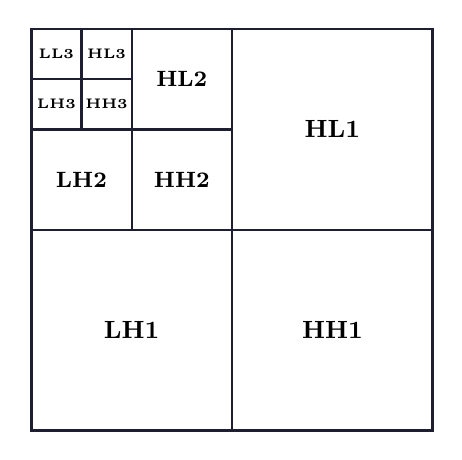
\begin{tikzpicture}[scale=0.85]
  % Boundary Box
  \draw[draw=mydark, line width=1pt] (0,0) rectangle (6,6);
  
  % Level 1 division
  \draw[line] (3,0) -- (3,6);
  \draw[line] (0,3) -- (6,3);
  \node[font=\small\bfseries] at (4.5, 4.5) {HL1};
  \node[font=\small\bfseries] at (1.5, 1.5) {LH1};
  \node[font=\small\bfseries] at (4.5, 1.5) {HH1};
  
  % Level 2 division
  \draw[line] (1.5,3) -- (1.5,6);
  \draw[line] (0,4.5) -- (3,4.5);
  \node[font=\footnotesize\bfseries] at (2.25, 5.25) {HL2};
  \node[font=\footnotesize\bfseries] at (0.75, 3.75) {LH2};
  \node[font=\footnotesize\bfseries] at (2.25, 3.75) {HH2};
  
  % Level 3 division
  \draw[line] (0.75,4.5) -- (0.75,6);
  \draw[line] (0,5.25) -- (1.5,5.25);
  \node[font=\tiny\bfseries] at (0.375, 5.625) {LL3};
  \node[font=\tiny\bfseries] at (1.125, 5.625) {HL3};
  \node[font=\tiny\bfseries] at (0.375, 4.875) {LH3};
  \node[font=\tiny\bfseries] at (1.125, 4.875) {HH3};
\end{tikzpicture}
\end{tcolorbox}

\subsection{Non-Separable Multi-dimensional Wavelets}
Separable transforms prioritize horizontal and vertical directions. \textbf{Non-separable 2D wavelets} use non-diagonal dilation matrices (like \textbf{Quincunx sampling}), splitting the frequency spectrum diagonally. This offers isotropic directional resolution and is less computationally redundant.

% ===============================================================================
\section{Wavelet Packets}
% ===============================================================================

\begin{tcolorbox}[defbox, title={\textbf{Definition of Wavelet Packets}}]
In a standard DWT, only the low-frequency approximation coefficients ($a_j$) are decomposed at each step. \textbf{Wavelet Packets (WP)} generalize this by recursively decomposing \textbf{both} approximation ($a_j$) and detail ($d_j$) coefficients, forming a \textbf{full binary tree} representation of the signal.
\end{tcolorbox}

\begin{tcolorbox}[tikzbox, title={Wavelet Packet (WP) vs. Standard DWT Trees}]
\centering
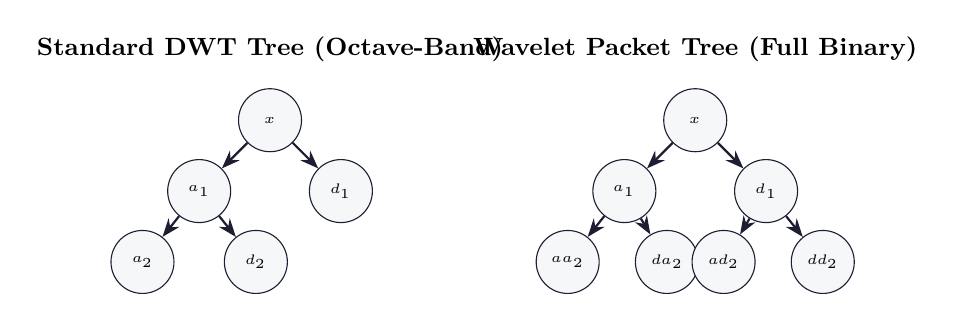
\begin{tikzpicture}[scale=0.9,
  node/.style={circle, draw=mydark, fill=mygray, minimum size=0.8cm, font=\tiny\bfseries}]
  
  % Standard DWT Tree
  \node at (1.5,2.5) {\small\bfseries Standard DWT Tree (Octave-Band)};
  \node[node] (s0) at (1.5,1.5) {$x$};
  \node[node] (sa1) at (0.5,0.5) {$a_1$};
  \node[node] (sd1) at (2.5,0.5) {$d_1$};
  \node[node] (sa2) at (-0.3,-0.5) {$a_2$};
  \node[node] (sd2) at (1.3,-0.5) {$d_2$};
  \draw[arrow] (s0) -- (sa1);
  \draw[arrow] (s0) -- (sd1);
  \draw[arrow] (sa1) -- (sa2);
  \draw[arrow] (sa1) -- (sd2);

  % Wavelet Packet Tree
  \node at (7.5,2.5) {\small\bfseries Wavelet Packet Tree (Full Binary)};
  \node[node] (w0) at (7.5,1.5) {$x$};
  \node[node] (wa1) at (6.5,0.5) {$a_1$};
  \node[node] (wd1) at (8.5,0.5) {$d_1$};
  \node[node] (wa2) at (5.7,-0.5) {$aa_2$};
  \node[node] (wad2) at (7.1,-0.5) {$da_2$};
  \node[node] (wda2) at (7.9,-0.5) {$ad_2$};
  \node[node] (wd2) at (9.3,-0.5) {$dd_2$};
  \draw[arrow] (w0) -- (wa1);
  \draw[arrow] (w0) -- (wd1);
  \draw[arrow] (wa1) -- (wa2);
  \draw[arrow] (wa1) -- (wad2);
  \draw[arrow] (wd1) -- (wda2);
  \draw[arrow] (wd1) -- (wd2);
\end{tikzpicture}
\tcbset{after={\color{black}}}
\end{tcolorbox}

\textbf{Advantages of Wavelet Packets:}
\begin{itemize}[leftmargin=*, itemsep=4.5pt]
  \item \textbf{Rich Spectral Breakdown:} Yields $2^J$ subbands at level $J$, dividing the frequency spectrum uniformly (equal-width subbands).
  \item \textbf{Best Basis Selection:} Using entropy metrics (like \textbf{Shannon entropy}), the algorithm selects the optimal path through the tree to maximize sparsity, matching the signal's specific frequency patterns.
\end{itemize}

\newpage
% ===============================================================================
\begin{center}
  {\large\bfseries\color{myred} Quick Revision --- Module 5}\\[3pt]
  {\small\color{mydark} Bi-orthogonal Wavelets $|$ PE-EC703C}
\end{center}
\noindent{\color{myred}\rule{\linewidth}{1.2pt}}
\vspace{4pt}
% ===============================================================================

\begin{tcolorbox}[formulabox, title={\textbf{Key Equations}}]
\renewcommand{\arraystretch}{1.35}
\begin{tabularx}{\linewidth}{B{5.0cm} X}
Bi-orthogonality Rel. & $\langle \phi(t), \tilde{\phi}(t-k) \rangle = \delta[k], \quad \langle \psi(t), \tilde{\psi}(t-k) \rangle = \delta[k]$ \\[4pt]
PR filter condition & $H_0(z)\tilde{H}_0(z^{-1}) + H_1(z)\tilde{H}_1(z^{-1}) = 2$ \\[4pt]
2D Approximation (LL) & $\Phi(x,y) = \phi(x)\phi(y)$ \\[4pt]
2D Horiz. Wavelet (HL) & $\Psi^H(x,y) = \phi(x)\psi(y)$ \\[4pt]
2D Vert. Wavelet (LH) & $\Psi^V(x,y) = \psi(x)\phi(y)$ \\[4pt]
2D Diag. Wavelet (HH) & $\Psi^D(x,y) = \psi(x)\psi(y)$
\end{tabularx}
\tcbset{after={\color{black}}}
\end{tcolorbox}

\begin{tcolorbox}[defbox, title={\textbf{One-Line Definitions}}]
\begin{itemize}[leftmargin=*, itemsep=3.5pt]
  \item \textbf{Bi-orthogonal Wavelet:} A wavelet system utilizing dual, cross-orthogonal scaling and wavelet bases for decomposition and reconstruction.
  \item \textbf{Linear Phase:} Filter characteristic indicating constant group delay, preventing signal phase distortion.
  \item \textbf{CDF 9/7 Wavelet:} A symmetric biorthogonal filter family used for lossy image compression in JPEG 2000.
  \item \textbf{Separable 2D DWT:} 2D transform implemented by running 1D transforms along rows and columns sequentially.
  \item \textbf{Non-separable Wavelet:} A 2D wavelet transform using multi-directional sampling grids (e.g. Quincunx).
  \item \textbf{Wavelet Packet:} Decompositions where both low-pass and high-pass branches are recursively filtered.
\end{itemize}
\end{tcolorbox}

\begin{tcolorbox}[exambox, title={\textbf{Frequently Asked / Viva Questions}}]
\begin{enumerate}[topsep=0pt, label=\textbf{Q\arabic*.}, itemsep=5pt]
  \item \Q{Why do we need bi-orthogonal wavelets in image processing?}
        In image processing, phase distortion must be avoided. Orthonormal wavelets (except Haar) cannot be symmetric (which is required for linear phase). Bi-orthogonal wavelets decouple decomposition and reconstruction, allowing filters to be symmetric and linear-phase while remaining compactly supported.

  \item \Q{What is the difference between CDF 9/7 and CDF 5/3 filters in JPEG 2000?}
        The CDF 9/7 filter has 9 analysis and 7 synthesis coefficients. It is used for lossy compression because it has high vanishing moments and excellent energy compaction. The CDF 5/3 filter has 5 analysis and 3 synthesis coefficients, uses integer coefficients, and is used for lossless compression.

  \item \Q{Explain separable 2D wavelet decomposition.}
        A separable 2D wavelet transform is computed by applying the 1D DWT horizontally along each row of the image, followed by applying the 1D DWT vertically along each column. This decomposes the image into four subbands: LL (approximation), LH (vertical details), HL (horizontal details), and HH (diagonal details).

  \item \Q{What is Quincunx sampling in multi-dimensional wavelets?}
        Quincunx sampling is a non-separable 2D downsampling scheme. It reduces the sampling grid by a factor of 2 in a diagonal checkerboard pattern. It provides isotropic frequency responses, avoiding the horizontal/vertical directional bias of separable transforms.

  \item \Q{How do Wavelet Packets differ from standard DWT?}
        A standard DWT only decomposes the approximation subband ($a_j$) at each level. A Wavelet Packet transform recursively decomposes both the approximation ($a_j$) and detail ($d_j$) subbands, generating a full binary tree. This provides higher spectral resolution at high frequencies.

  \item \Q{What is "best basis selection" in Wavelet Packets?}
        Since Wavelet Packets generate a redundant binary tree, we must select the most efficient subbands. The best basis algorithm evaluates the entropy (e.g. Shannon entropy) of each node and prunes the tree to minimize representation cost.
\end{enumerate}
\end{tcolorbox}

\begin{tcolorbox}[tikzbox, title={\textbf{Summary Comparison: DWT vs. Wavelet Packets}}]
\par\noindent
{\renewcommand{\arraystretch}{1.4}%
\begin{tabularx}{\linewidth}{|B{3.2cm}|Y|Y|}
\hline
\textbf{Feature} & \textbf{Standard DWT} & \textbf{Wavelet Packets (WP)} \\
\hline
\textbf{Decomposition Tree} & Octave-band (unbalanced tree). & Full binary tree (symmetrical). \\
\hline
\textbf{Subbands at Level $J$} & $3J+1$ subbands. & $2^J$ subbands. \\
\hline
\textbf{Frequency Resolution} & Logarithmic (narrow at low frequencies). & Uniform (equal bandwidth bands). \\
\hline
\textbf{Adaptivity} & Rigid (fixed octaves). & Highly adaptive (best basis selection). \\
\hline
\textbf{Sparsity for Curves} & Poor (requires many coefficients). & Poor (struggles with curved features). \\
\hline
\end{tabularx}}
\end{tcolorbox}


% -- Module 6 -----------------------------------------------------------------
\modulestart{6}{Transform Coding and Data Compression}

\section{Transform Coding and Data Compression}
% ===============================================================================

Data compression reduces transmission bandwidth and storage requirements. In \textbf{Transform Coding}, a mathematical transform maps spatial/temporal domain signal values to a frequency-like domain, where the coefficients are less correlated and easier to compress.

\subsection{Principles of Transform Coding}
Transform coding relies on three core steps:
\begin{enumerate}[leftmargin=*, itemsep=4pt]
  \item \textbf{Transform:} De-correlates the signal data, packing most of the energy into a few high-magnitude coefficients (Energy Compaction).
  \item \textbf{Quantization:} Converts continuous or high-precision coefficients to discrete levels. This is a lossy step where small, high-frequency coefficients (representing details less perceptible to human eyes/ears) are rounded to zero.
  \item \textbf{Entropy Coding:} Applies lossless compression (e.g., Huffman or Arithmetic coding) to the quantized symbols, mapping more frequent values to shorter codewords.
\end{enumerate}

\subsection{Image and Audio Compression: DWT/DTWT vs. DCT (JPEG 2000 vs. JPEG)}
For discrete-time sequences (such as digital audio and images), the Discrete Wavelet Transform is implemented as the \textbf{Discrete-Time Wavelet Transform (DTWT)} using digital filter banks.
\begin{itemize}[leftmargin=*, itemsep=4pt]
  \item \textbf{JPEG (Discrete Cosine Transform):} Splits an image into non-overlapping $8 \times 8$ blocks and applies 2D DCT to each block. At high compression ratios, discarding high-frequency coefficients creates artificial grid-like discontinuities at block boundaries, known as \textbf{blocking artifacts}.
  \item \textbf{JPEG 2000 (Discrete Wavelet Transform):} Applies DWT globally over the entire image (or large tile regions). This eliminates blocking artifacts, resulting in graceful, blurry degradation rather than grid patterns. 
  \item \textbf{Key Advantages of JPEG 2000 over JPEG:}
        \begin{itemize}[leftmargin=*, itemsep=2.5pt, topsep=2pt]
          \item \textbf{No Blocking Artifacts:} Smooth, visually superior reconstruction at low bitrates.
          \item \textbf{Progressive Transmission:} Single bitstream contains multiple resolutions and quality layers. A low-resolution thumbnail is decoded first, followed by details as more data arrives.
          \item \textbf{Region of Interest (ROI) Coding:} Particular regions of an image (e.g., a tumor in a medical scan) can be encoded with higher precision than the background.
          \item \textbf{Unified Lossless and Lossy:} Uses the CDF 5/3 filter bank for lossless compression and the CDF 9/7 filter bank for lossy compression.
        \end{itemize}
\end{itemize}

\par\noindent
{\renewcommand{\arraystretch}{1.4}%
\begin{tabularx}{\linewidth}{|B{3.5cm}|Y|Y|}
\hline
\textbf{Feature} & \textbf{Standard JPEG (DCT-based)} & \textbf{JPEG 2000 (DWT-based)} \\
\hline
\textbf{Core Transform} & Block-based Discrete Cosine Transform (DCT). & Discrete Wavelet Transform (DWT). \\
\hline
\textbf{Processing Unit} & Fixed $8 \times 8$ pixel blocks. & Entire image or large tile regions. \\
\hline
\textbf{Compression Ratio} & Poor quality at ratios $> 30:1$ (blocks visible). & Excellent quality at high ratios ($> 100:1$). \\
\hline
\textbf{Artifact Type} & Blocking artifacts (grid patterns) and mosquito noise. & Blurring and ringing artifacts around edges. \\
\hline
\textbf{Scalability} & Not natively supported (needs separate files). & Resolution and quality scalability in one stream. \\
\hline
\textbf{Entropy Coder} & Huffman Coding. & Context-adaptive EBCOT (Arithmetic Coding). \\
\hline
\end{tabularx}}

\subsection{Audio Coding and Video Coding}
\begin{itemize}[leftmargin=*, itemsep=4pt]
  \item \textbf{Audio Coding:} The human ear acts as a spectrum analyzer. Wavelet-based audio coders exploit this multi-resolution structure. By dividing the audio spectrum into subbands matching the ear's \textbf{critical bands}, subband coding allocates bits dynamically based on psychoacoustic masking (louder sounds mask quieter adjacent frequencies).
  \item \textbf{Video Coding:} Standard video codecs (H.264/H.265) utilize block-based motion estimation and DCT. Wavelet-based video coding uses DWT on individual frames or applies a \textbf{3D DWT} (spatial $x$-$y$ DWT + temporal $t$ DWT) to compress spatial and motion information simultaneously, avoiding motion compensation loops.
\end{itemize}

% ===============================================================================
\section{Wavelet De-noising and Image Processing}
% ===============================================================================

\subsection{Wavelet De-noising (Hard vs. Soft Thresholding)}
Consider a noisy signal model:
$$y_i = x_i + \sigma z_i, \quad i = 1, 2, \dots, N$$
where $y_i$ is the observed noisy signal, $x_i$ is the clean signal, $\sigma$ is the noise standard deviation, and $z_i \sim \mathcal{N}(0, 1)$ is additive white Gaussian noise (AWGN).

Since DWT is a linear orthogonal transform, the noise remains white and spread evenly across all coefficients, whereas the signal energy is concentrated into a few large wavelet coefficients. Denoising is achieved by thresholding the DWT coefficients.

\begin{tcolorbox}[formulabox, title={\textbf{Hard and Soft Thresholding Formulations}}]
Let $w$ represent a wavelet coefficient, and $\lambda$ be the threshold limit ($\lambda > 0$).
\begin{enumerate}[leftmargin=*, itemsep=4pt, label=\arabic*.]
  \item \textbf{Hard Thresholding:} Sets coefficients below the threshold to zero, keeping the others unchanged:
        $$\eta_\lambda^{\text{hard}}(w) = \begin{cases} w, & |w| > \lambda \\ 0, & |w| \le \lambda \end{cases}$$
  \item \textbf{Soft Thresholding (Wavelet Shrinkage):} Sets coefficients below the threshold to zero, and shrinks the remaining coefficients towards zero:
        $$\eta_\lambda^{\text{soft}}(w) = \text{sgn}(w)\max(|w| - \lambda, 0)$$
\end{enumerate}
\tcbset{after={\color{black}}}
\end{tcolorbox}

\begin{itemize}[leftmargin=*, itemsep=4.5pt]
  \item \textbf{Comparison:} Hard thresholding preserves edge sharpness but can introduce spurious oscillations (pseudo-Gibbs phenomena) due to the discontinuity in the thresholding function. Soft thresholding is continuous, yielding smoother denoised signals, but it introduces a bias by scaling down large coefficients, which slightly blurs sharp peaks.
\end{itemize}

\subsection{Threshold Selection Rules}
\begin{itemize}[leftmargin=*, itemsep=4.5pt]
  \item \textbf{VisuShrink (Universal Threshold):} Uses a global threshold derived by Donoho and Johnstone:
        $$\lambda_{\text{univ}} = \sigma \sqrt{2 \ln N}$$
        where $N$ is the length of the signal. It guarantees with high probability that the maximum noise coefficient is below $\lambda$. However, for large $N$, $\lambda_{\text{univ}}$ becomes large, causing over-smoothing (loss of fine details). The noise variance $\sigma$ is estimated from the median absolute deviation (MAD) of the finest detail subband ($HH_1$):
        $$\hat{\sigma} = \frac{\text{median}(|w_{j,k}|)}{0.6745}, \quad w_{j,k} \in \text{finest subband}$$
  \item \textbf{SureShrink:} An adaptive, subband-dependent thresholding method. For each subband, it selects a threshold $\lambda$ that minimizes \textbf{Stein's Unbiased Risk Estimate (SURE)}, optimizing the mean squared error (MSE) estimate.
\end{itemize}

\begin{tcolorbox}[tikzbox, title={Wavelet-Based Denoising Process Flow}]
\centering
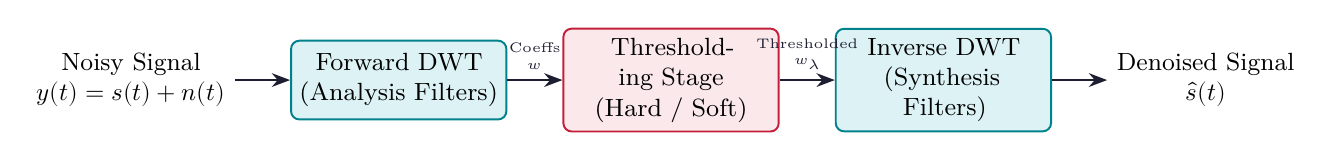
\begin{tikzpicture}[node distance=1.0cm and 0.8cm, auto]
  \node (input) [align=center, font=\small] {Noisy Signal\\$y(t) = s(t) + n(t)$};
  \node (dwt) [block, right=0.7cm of input] {Forward DWT\\(Analysis Filters)};
  \node (thresh) [redblock, right=0.7cm of dwt] {Thresholding Stage\\(Hard / Soft)};
  \node (idwt) [block, right=0.7cm of thresh] {Inverse DWT\\(Synthesis Filters)};
  \node (output) [right=0.7cm of idwt, align=center, font=\small] {Denoised Signal\\$\hat{s}(t)$};

  \draw [arrow] (input) -- (dwt);
  \draw [arrow] (dwt) -- node[above, font=\tiny, align=center] {Coeffs\\$w$} (thresh);
  \draw [arrow] (thresh) -- node[above, font=\tiny, align=center] {Thresholded\\$w_\lambda$} (idwt);
  \draw [arrow] (idwt) -- (output);
\end{tikzpicture}
\end{tcolorbox}

\subsection{Speckle Removal (Homomorphic Wavelet Filtering)}
Speckle is a high-frequency multiplicative noise common in coherent imaging systems like Synthetic Aperture Radar (SAR) and Ultrasound:
$$y = x \cdot n$$
where $y$ is the observed image, $x$ is the noise-free image, and $n$ is the speckle noise.
Standard denoising assumes additive noise. To resolve this, \textbf{Homomorphic Filtering} is applied:
\begin{enumerate}[leftmargin=*, itemsep=4pt]
  \item Take the logarithm of the noisy image to convert multiplicative noise into additive noise:
        $$\ln(y) = \ln(x) + \ln(n) \implies y' = x' + n'$$
  \item Apply DWT to $y'$, perform thresholding on the detail subbands, and apply IDWT to get the denoised estimate $\hat{x}'$.
  \item Exponentiate the result to return to the original scale:
        $$\hat{x} = \exp(\hat{x}')$$
\end{enumerate}

\subsection{Edge Detection and Object Isolation}
\begin{itemize}[leftmargin=*, itemsep=4.5pt]
  \item \textbf{Edge Detection:} Sharp changes in image intensity (edges) correspond to local maxima of the wavelet transform modulus at fine scales. By observing coefficients across multiple scales, we can distinguish true edges (which persist across scales) from random noise (which rapidly decays at coarser scales).
  \item \textbf{Image Fusion:} Combines complementary information from multiple images of the same scene (e.g., multi-focus or infrared/visible cameras). The source images are decomposed using DWT. The coefficient subbands are fused:
        \begin{itemize}[leftmargin=*, itemsep=2.5pt, topsep=2pt]
          \item \textbf{LL (Approximation) Coefficients:} Typically averaged to preserve average illumination.
          \item \textbf{Detail Coefficients (LH, HL, HH):} Selected using a "maximum absolute value" rule, as larger coefficients correspond to sharper, in-focus features.
        \end{itemize}
        Applying the IDWT to the fused coefficients yields a single high-quality composite image.
\end{itemize}

% ===============================================================================
\section{Discrete Wavelet Multi-Tone Modulation (DWMT)}
% ===============================================================================

\begin{tcolorbox}[defbox, title={\textbf{Definition of DWMT}}]
\textbf{Discrete Wavelet Multi-Tone (DWMT)} modulation is a multicarrier communication technique that uses Orthogonal Wavelet Filter Banks (specifically, Cosine-Modulated Filter Banks or Synthesis/Analysis Wavelet filters) as subcarrier generators instead of the DFT/IDFT used in standard OFDM.
\end{tcolorbox}

In standard \textbf{OFDM (Orthogonal Frequency Division Multiplexing)}, subcarriers are shaped like sinc functions because they are modulated by a rectangular window. This yields high spectral sidelobes ($-13\text{ dB}$). Any frequency offset causes \textbf{Inter-Carrier Interference (ICI)}, requiring a \textbf{Cyclic Prefix (CP)} guard interval which reduces spectral efficiency by $10\text{--}25\%$.

\subsubsection{Advantages of DWMT over OFDM:}
\begin{enumerate}[leftmargin=*, itemsep=4pt]
  \item \textbf{Low Sidelobes:} Wavelet filters have excellent spectral containment, with sidelobes decaying much faster than $-13\text{ dB}$ (often below $-40\text{ dB}$).
  \item \textbf{No Cyclic Prefix:} Because spectral overlap between non-adjacent subcarriers is negligible, DWMT does not require a cyclic prefix. This saves transmission bandwidth.
  \item \textbf{High ICI/ISI Immunity:} The high stop-band attenuation of wavelet filters makes DWMT robust against narrowband interference and multipath channel distortions.
\end{enumerate}

\newpage
% ===============================================================================
\begin{center}
  {\large\bfseries\color{myred} Quick Revision --- Module 6}\\[3pt]
  {\small\color{mydark} Wavelet Transform and Applications $|$ PE-EC703C}
\end{center}
\noindent{\color{myred}\rule{\linewidth}{1.2pt}}
\vspace{4pt}
% ===============================================================================

\begin{tcolorbox}[formulabox, title={\textbf{Key Equations}}]
\renewcommand{\arraystretch}{1.35}
\begin{tabularx}{\linewidth}{B{5.0cm} X}
Hard Thresholding & $\eta_\lambda^{\text{hard}}(w) = \begin{cases} w, & |w| > \lambda \\ 0, & |w| \le \lambda \end{cases}$ \\[12pt]
Soft Thresholding & $\eta_\lambda^{\text{soft}}(w) = \text{sgn}(w)\max(|w| - \lambda, 0)$ \\[4pt]
Universal Threshold & $\lambda_{\text{univ}} = \sigma \sqrt{2 \ln N}$ \\[4pt]
Noise Variance Estimate & $\hat{\sigma} = \frac{\text{median}(|w_{j,k}|)}{0.6745} \quad (w_{j,k} \in \text{finest subband } HH_1)$
\end{tabularx}
\tcbset{after={\color{black}}}
\end{tcolorbox}

\begin{tcolorbox}[defbox, title={\textbf{One-Line Definitions}}]
\begin{itemize}[leftmargin=*, itemsep=3.5pt]
  \item \textbf{Energy Compaction:} Concentrate signal representation into a small number of large coefficients.
  \item \textbf{Blocking Artifacts:} Grid-like boundaries visible at low bitrates in block-based DCT compression.
  \item \textbf{Wavelet Shrinkage:} Noise reduction method that attenuates coefficients toward zero (soft thresholding).
  \item \textbf{VisuShrink:} Denoising method using the universal threshold $\sigma \sqrt{2 \ln N}$ to remove noise with high probability.
  \item \textbf{SureShrink:} Adaptive denoising scheme minimizing Stein's Unbiased Risk Estimate for each subband.
  \item \textbf{Homomorphic Filter:} Transform mapping multiplicative noise to additive noise via log operations.
  \item \textbf{DWMT Modulation:} Multicarrier modulation using wavelet synthesis/analysis filter banks instead of DFT.
\end{itemize}
\end{tcolorbox}

\begin{tcolorbox}[exambox, title={\textbf{Frequently Asked / Viva Questions}}]
\begin{enumerate}[topsep=0pt, label=\textbf{Q\arabic*.}, itemsep=5pt]
  \item \Q{Why does JPEG 2000 perform better than standard JPEG at low bitrates?}
        Standard JPEG uses block-based DCT ($8 \times 8$), which causes blocking artifacts due to independent processing of boundaries. JPEG 2000 uses DWT globally on the entire image, which yields no block borders and results in a graceful blur at low bitrates.

  \item \Q{Compare hard and soft thresholding in terms of visual quality and math.}
        Hard thresholding is discontinuous and keeps coefficients larger than $\lambda$ unchanged, which preserves sharp edges but can create pseudo-Gibbs oscillations. Soft thresholding is continuous and reduces coefficients by $\lambda$, which yields smoother signals but introduces bias and blurs sharp peaks.

  \item \Q{What is the universal threshold in VisuShrink, and what is its drawback?}
        $\lambda_{\text{univ}} = \sigma \sqrt{2 \ln N}$. Its drawback is that as signal length $N$ increases, the threshold becomes excessively large. This removes almost all noise but also removes true high-frequency signal details, causing over-smoothing.

  \item \Q{How do we estimate the noise variance $\sigma$ in practical image denoising?}
        It is estimated from the median absolute deviation (MAD) of the finest detail subband coefficients ($HH_1$): $\hat{\sigma} = \text{median}(|w_{j,k}|) / 0.6745$.

  \item \Q{Explain the homomorphic wavelet denoising workflow for speckle noise.}
        Speckle is multiplicative ($y = x \cdot n$). We apply a logarithmic transform: $\ln(y) = \ln(x) + \ln(n)$ to convert it to additive noise. We then apply DWT, perform wavelet thresholding, apply IDWT, and finally exponentiate the result.

  \item \Q{How is DWT used for image fusion?}
        Multiple source images are decomposed by DWT. The LL (approximation) coefficients are averaged to preserve illumination, and the detail coefficients (LH, HL, HH) are fused by taking the maximum absolute value (which preserves sharp details and focus). The fused image is reconstructed using IDWT.

  \item \Q{What are the advantages of DWMT over OFDM?}
        DWMT uses wavelet filter banks which have much lower sidelobes than OFDM's sinc subcarriers. This reduces Inter-Carrier Interference (ICI) and eliminates the need for a Cyclic Prefix (CP), increasing spectral efficiency.
\end{enumerate}
\end{tcolorbox}

\begin{tcolorbox}[tikzbox, title={\textbf{JPEG vs. JPEG 2000 Comparison Matrix}}]
\par\noindent
{\renewcommand{\arraystretch}{1.4}%
\begin{tabularx}{\linewidth}{|B{3.2cm}|Y|Y|}
\hline
\textbf{Feature} & \textbf{Standard JPEG (DCT-based)} & \textbf{JPEG 2000 (DWT-based)} \\
\hline
\textbf{Core Transform} & Block-based Discrete Cosine Transform (DCT). & Discrete Wavelet Transform (DWT). \\
\hline
\textbf{Processing Unit} & Fixed $8 \times 8$ pixel blocks. & Entire image or large tile regions. \\
\hline
\textbf{Compression Ratio} & Poor quality at ratios $> 30:1$ (blocks visible). & Excellent quality at high ratios ($> 100:1$). \\
\hline
\textbf{Artifact Type} & Blocking artifacts (grid patterns) and mosquito noise. & Blurring and ringing artifacts around edges. \\
\hline
\textbf{Scalability} & Not natively supported (needs separate files). & Resolution and quality scalability in one stream. \\
\hline
\textbf{Entropy Coder} & Huffman Coding. & Context-adaptive EBCOT (Arithmetic Coding). \\
\hline
\end{tabularx}}
\end{tcolorbox}


% -- Module 7 -----------------------------------------------------------------
\modulestart{7}{Limitations of Wavelets in Two Dimensions}

\section{Limitations of Wavelets in Two Dimensions}
% ===============================================================================

Standard 2D wavelets are created by tensor products of 1D wavelets (separable DWT). Their spatial support is square (isotropic). While excellent at representing point singularities, they struggle to capture \textbf{line or curve singularities} (such as edges in an image). 

To represent a smooth curve, 2D wavelets require a large number of coefficients at fine scales, failing to achieve optimal \textbf{sparsity}. This limitation is known as the \textit{curse of dimensionality} for directional features.

% ===============================================================================
\section{Ridgelet Transform}
% ===============================================================================

The continuous Ridgelet transform is designed specifically to capture line singularities in 2D. A ridgelet function in $\mathbb{R}^2$ is defined by scaling ($a$), translating ($b$), and rotating ($\theta$):
$$\psi_{a,b,\theta}(x, y) = a^{-1/2} \psi\left(\frac{x \cos\theta + y \sin\theta - b}{a}\right)$$
Here, the wavelets are constant along the lines $x \cos\theta + y \sin\theta = \text{constant}$ (ridges).

\textbf{Relationship to Radon Transform:}
The Ridgelet transform can be implemented by first taking the \textbf{Radon Transform} of the image $f(x,y)$ (which maps line integrals to points) and then applying a \textbf{1D Wavelet Transform} along the radial direction:
$$\text{Ridgelet Transform} = \text{1D DWT} \circ \text{Radon Transform}$$

% ===============================================================================
\section{Curvelet Transform}
% ===============================================================================

While Ridgelets handle straight line singularities, real-world images contain curved edges. The \textbf{Curvelet Transform} generalizes Ridgelets to handle curves by partitioning the image into small local patches, and applying a local Ridgelet transform to each patch.

\subsection{Parabolic Scaling of Curvelets}
A key mathematical property of curvelets is \textbf{Parabolic Scaling}, which governs the relationship between the width and length of their spatial support at scale $j$:
\begin{tcolorbox}[formulabox, title={\textbf{Parabolic Scaling Law}}]
$$\text{width} \approx \text{length}^2 \quad \implies \quad \text{width} \propto 2^{-j}, \quad \text{length} \propto 2^{-j/2}$$
\tcbset{after={\color{black}}}
\end{tcolorbox}
At fine scales, curvelets become highly needle-like (highly anisotropic), allowing them to align perfectly with curved edge structures.

\subsection{Digital Curvelet Transform Implementation}
Two fast algorithms exist for the discrete curvelet transform:
\begin{enumerate}[leftmargin=*, itemsep=4pt]
  \item \textbf{Unequally Spaced Fast Fourier Transform (USFFT):} Samples the Fourier transform of the image along a polar-like grid of wedges.
  \item \textbf{Wrapping Algorithm:} Wraps Fourier wedges into a rectangular grid around the origin, which is faster and computationally more efficient.
\end{enumerate}

\begin{tcolorbox}[tikzbox, title={Ridgelet vs. Curvelet Frequency Domain Partitioning}]
\centering
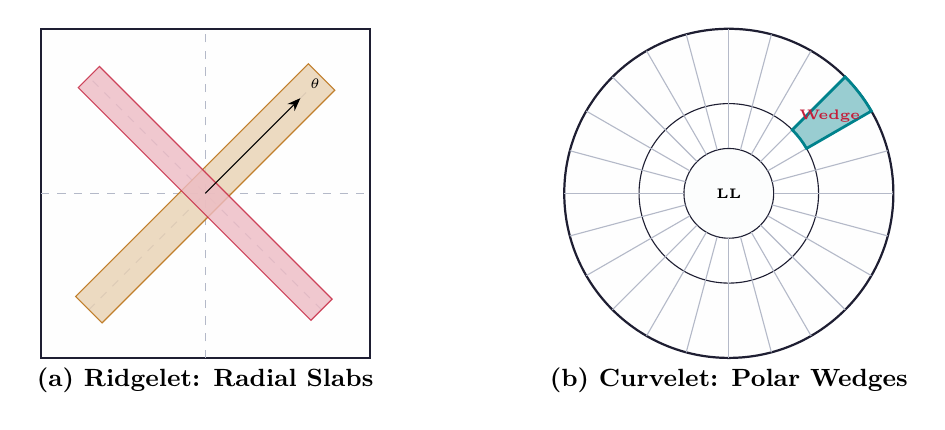
\begin{tikzpicture}[scale=0.95]
  % Ridgelet Partitioning
  \begin{scope}[xshift=-3.5cm]
    \draw[draw=mydark, fill=mygray!10, line width=0.8pt] (-2.2,-2.2) rectangle (2.2,2.2);
    % Radial lines
    \foreach \angle in {0, 45, 90, 135} {
      \draw[dashed, mgframe] (\angle:-2.2cm) -- (\angle:2.2cm);
    }
    % Draw radial slabs
    \draw[fill=myamber!30, draw=myamber, opacity=0.8, rotate=45] (-2.2,-0.25) rectangle (2.2,0.25);
    \draw[fill=myred!30, draw=myred, opacity=0.8, rotate=135] (-2.2,-0.2) rectangle (2.2,0.2);
    \node at (0,-2.5) [font=\small\bfseries] {(a) Ridgelet: Radial Slabs};
    \draw[-Stealth, thin] (0,0) -- (45:1.8cm) node[above right, font=\tiny] {$\theta$};
  \end{scope}

  % Curvelet Partitioning
  \begin{scope}[xshift=3.5cm]
    \draw[draw=mydark, fill=mygray!10, line width=0.8pt] (0,0) circle (2.2cm);
    \draw[fill=white, draw=mydark] (0,0) circle (1.2cm);
    \draw[fill=mygray!30, draw=mydark] (0,0) circle (0.6cm);
    
    % Radial divisions
    \foreach \angle in {0, 15, 30, 45, 60, 75, 90, 105, 120, 135, 150, 165, 180, 195, 210, 225, 240, 255, 270, 285, 300, 315, 330, 345} {
      \draw[mgframe, thin] (\angle:0.6cm) -- (\angle:2.2cm);
    }
    
    % Highlight one Curvelet wedge (Parabolic scaling: length = r*dtheta, width = dr)
    \draw[fill=myteal!40, draw=myteal, line width=1pt] (30:1.2cm) arc (30:45:1.2cm) -- (45:2.2cm) arc (45:30:2.2cm) -- cycle;
    \node[font=\tiny\bfseries, color=myred] at (37.5:1.7cm) {Wedge};
    
    \node at (0,-2.5) [font=\small\bfseries] {(b) Curvelet: Polar Wedges};
    \node at (0,0) [font=\tiny\bfseries] {LL};
  \end{scope}
\end{tikzpicture}
\end{tcolorbox}

% ===============================================================================
\section{Properties and Applications of Ridgelets and Curvelets}
% ===============================================================================

\begin{itemize}[leftmargin=*, itemsep=4.5pt]
  \item \textbf{Properties:} 
        \begin{itemize}[leftmargin=*, itemsep=2.5pt, topsep=2pt]
          \item \textbf{High Directional Sensitivity:} Support orientations increase at finer scales.
          \item \textbf{Optimal Sparsity:} Curvelets represent curved edges with very few non-zero coefficients compared to wavelets.
        \end{itemize}
  \item \textbf{Applications:}
        \begin{itemize}[leftmargin=*, itemsep=2.5pt, topsep=2pt]
          \item \textbf{Seismic Data Processing:} Identifying straight and curved geological faults.
          \item \textbf{CT/MRI Reconstruction:} Solving tomographic reconstruction problems from radon projections.
          \item \textbf{Directional Image Denoising:} Removing noise while preserving sharp curved edges.
        \end{itemize}
\end{itemize}

\newpage
% ===============================================================================
\begin{center}
  {\large\bfseries\color{myred} Quick Revision --- Module 7}\\[3pt]
  {\small\color{mydark} Beyond Wavelet $|$ PE-EC703C}
\end{center}
\noindent{\color{myred}\rule{\linewidth}{1.2pt}}
\vspace{4pt}
% ===============================================================================

\begin{tcolorbox}[formulabox, title={\textbf{Key Equations}}]
\renewcommand{\arraystretch}{1.35}
\begin{tabularx}{\linewidth}{B{5.0cm} X}
Ridgelet Transform & $\psi_{a,b,\theta}(x, y) = a^{-1/2} \psi\left(\frac{x \cos\theta + y \sin\theta - b}{a}\right)$ \\[12pt]
Parabolic Scaling Law & $\text{width} \approx \text{length}^2 \implies \text{width} \propto 2^{-j}, \; \text{length} \propto 2^{-j/2}$
\end{tabularx}
\tcbset{after={\color{black}}}
\end{tcolorbox}

\begin{tcolorbox}[defbox, title={\textbf{One-Line Definitions}}]
\begin{itemize}[leftmargin=*, itemsep=3.5pt]
  \item \textbf{Anisotropic:} Having properties that differ depending on the direction of measurement (e.g., curvelet shape).
  \item \textbf{Radon Transform:} Mathematical integral projection mapping line integrals of a 2D function into 1D profiles.
  \item \textbf{Ridgelet Transform:} Directional 2D transform mapping straight line singularities to point-like representations.
  \item \textbf{Curvelet Transform:} Directional multiscale transform optimized for curved edge singularities.
  \item \textbf{Wrapping Algorithm:} Fast discrete curvelet transform that wraps Fourier wedges into a rectangular grid.
  \item \textbf{USFFT Algorithm:} Fast discrete curvelet transform that uses unequally spaced fast Fourier projections.
\end{itemize}
\end{tcolorbox}

\begin{tcolorbox}[exambox, title={\textbf{Frequently Asked / Viva Questions}}]
\begin{enumerate}[topsep=0pt, label=\textbf{Q\arabic*.}, itemsep=5pt]
  \item \Q{Why are standard wavelets inefficient at representing curved edges in 2D?}
        Separable 2D wavelets have square spatial support. Representing a smooth curved edge requires many small wavelets along the curve at fine scales, which destroys sparsity.

  \item \Q{How is the Ridgelet transform implemented using the Radon transform?}
        The Ridgelet transform is implemented by first applying the Radon transform to project line integrations into 1D profiles, followed by a 1D continuous wavelet transform along those radial profiles.

  \item \Q{What is the parabolic scaling property of curvelets?}
        Curvelets scale such that $\text{width} \approx \text{length}^2$ (i.e. at scale $2^{-j}$, the width is $2^{-j}$ and length is $2^{-j/2}$). This anisotropic, needle-like shape allows curvelets to trace curved edges efficiently.

  \item \Q{Explain the two primary digital curvelet transform algorithms.}
        \begin{itemize}[leftmargin=*, itemsep=1pt, topsep=2pt]
          \item \textbf{USFFT:} Computes spatial coordinates on an irregular polar-like grid in the frequency domain.
          \item \textbf{Wrapping:} Wraps rectangular frequency wedges into a standard rectangular grid to allow fast FFT processing.
        \end{itemize}

  \item \Q{What are the primary applications of Ridgelets and Curvelets?}
        They are used in seismic data processing, CT/MRI tomographic reconstruction, and denoising of images with dominant curved structures, where wavelets would blur the edges.
\end{enumerate}
\end{tcolorbox}

\begin{tcolorbox}[tikzbox, title={\textbf{Multi-Resolution Feature Representation Comparison}}]
\par\noindent
{\renewcommand{\arraystretch}{1.45}%
\begin{tabularx}{\linewidth}{|B{3.0cm}|Y|Y|Y|}
\hline
\textbf{Property} & \textbf{Wavelet Transform} & \textbf{Ridgelet Transform} & \textbf{Curvelet Transform} \\
\hline
\textbf{Dimension} & 1D, 2D, or Multi-D. & 2D (or higher). & 2D (or higher). \\
\hline
\textbf{Optimal For} & Point singularities. & Straight line singularities. & Curved singularities (edges). \\
\hline
\textbf{Support Geometry} & Isotropic (square). & Line-like (infinite slabs). & Needle-like (parabolic wedges). \\
\hline
\textbf{Directionality} & 3 fixed directions in 2D. & Continuous angle $\theta$. & Multi-directional (scale-dependent). \\
\hline
\textbf{Fourier Tiling} & Concentric dyadic squares. & Radial strips. & Polar-like wedges. \\
\hline
\end{tabularx}}
\end{tcolorbox}


\end{document}
